% This is LLNCS.DEM the demonstration file of
% the LaTeX macro package from Springer-Verlag
% for Lecture Notes in Computer Science,
% version 2.4 for LaTeX2e as of 16. April 2010
%
\documentclass{llncs}
%
\usepackage[table]{xcolor}
\usepackage{cite}
\usepackage{multirow}
\usepackage{hhline}
\usepackage{caption}
\usepackage{makecell}
\usepackage{ragged2e}
\usepackage{parskip}
\usepackage{wrapfig}
\usepackage{array}
\usepackage{float}
\usepackage[english]{babel}
\usepackage{lipsum}
\usepackage{subcaption}
\usepackage{graphicx}
\graphicspath{{images/}} 
\usepackage[linesnumbered,ruled]{algorithm2e}
\usepackage{courier}
\usepackage{hyperref}
\hypersetup{colorlinks=true,allcolors=blue}
\usepackage{listings}
\usepackage{float}
\lstset{
    basicstyle=\ttfamily,
    frame=none, 
    breaklines=true,
    numbers=left,
    xleftmargin=2.5em,
    framexleftmargin=0em,
    emphstyle=\textbf,
    float=t
}
\lstdefinestyle{ocl}{
    emph={
        context, inv
    }
}
\lstdefinestyle{cbp}{
    basicstyle=\ttfamily\scriptsize,
    emph={
        session, create, type,
        set, to, add, hire
    }
}
\lstdefinestyle{xmi}{
    basicstyle=\ttfamily\scriptsize,
    emph={
        Node, children
    }
}
\lstdefinestyle{xml}{
    basicstyle=\ttfamily\scriptsize,
    emph={
        register, create, add, to, resource, at,
        from, eattribute, remove, ereference,
        set, unset, session, Roy, Jen,
        Moss, Richmond
    }
}
\lstdefinestyle{java}{
    basicstyle=\ttfamily\scriptsize,
    emph={
        case, $unset$,
        instanceof, else, if, void,
        new, UnsetEAttributeEvent,
        UnsetEReferenceEvent,
        @override, public, class, extends
    }
}
\lstdefinestyle{eol}{
    basicstyle=\ttfamily\scriptsize,
    emph={
        var, new, for, in, create, set, with, type, at,
        unset, to, add, remove, delete, register, move,
        from, position, from, move-within, session, \.
    }
}

% $ChangeHybridEventAdapter$

\hyphenation{op-tical net-works semi-conduc-tor Hybrid-Change-Event-Adapter Hybrid-XMI-Change-Event-Adapater
    Hybrid-Neo-EMF-Change-Event-Adapater change-Events Change-Event-Adapter EContent-Adapter notify-Changed Hybrid-Resource Resource-Impl state-Based-Resource cbp-Output-Stream Output-Stream Hybrid-Change-Event-Adapater Output-Stream Hybrid-XMI-Resource-Impl Hybrid-Neo-EMF-Resource-Impl Persistence-Resource change-Events
}

\definecolor{gray1}{gray}{0.90}
\definecolor{gray2}{gray}{0.95}


\begin{document}
\renewcommand{\thelstlisting}{\arabic{lstlisting}}
\renewcommand{\labelitemi}{$\bullet$}
\newcommand{\dk}[1]{\textbf{[DK: #1]}}
\newcommand{\And}{\textnormal{\textbf{and }}}
\newcommand{\Is}{\textnormal{\textbf{is }}}
\newcommand{\Not}{\textnormal{\textbf{not }}}

\title{Harnessing Change-based Persistence to Optimise Model Comparison}
%
\titlerunning{Harnessing Change-based Persistence to Optimise Model Comparison}  % abbreviated title (for running head)
%     also used for the TOC unless
%     \toctitle is used
%
\author{
Alfa Yohannis \and Horacio Hoyos Rodriguez$^{*}$ \and Fiona Polack$^{**}$ \and \\ Dimitris Kolovos
}

%\author{
%Alfa Yohannis$^{1,3}$ \and Horacio Hoyos Rodriguez$^{*1}$ \and Fiona Polack$^{**2}$ \and \\ Dimitris Kolovos$^{1}$
%}
%
\authorrunning{
Alfa Yohannis et al.
} % abbreviated author list (for running head)
%
%%%% list of authors for the TOC (use if author list has to be modified)
%\tocauthor{Alfa Yohannis,Horacio Hoyos Rodriguez, Fiona Polack, Dimitris Kolovos}
%\institute{anonym}

\institute{Department of Computer Science, University of York, United Kingdom\\
    $^{**}$School of Computing and Maths, Keele University, United Kingdom\\
\email{\{ary506, dimitris.kolovos\}@york.ac.uk
\\$^{*}$horacio\_hoyos\_rodriguez@ieee.org
\\$^{**}$f.a.c.polack@keele.ac.uk}}

%\institute{$^{1}$Department of Computer Science, University of York, United Kingdom\\
%    $^{2}$School of Computing and Maths, Keele University, United Kingdom\\
%    $^{3}$Department of Computer Science, Institut Teknologi dan Bisnis Kalbis, Indonesia\\
%    \email{\{ary506, dimitris.kolovos\}@york.ac.uk
%        \\$^{*}$horacio\_hoyos\_rodriguez@ieee.org
%        \\$^{**}$f.a.c.polack@keele.ac.uk}}

\maketitle      % typeset the title of the contribution

%The first states the problem. The second states why the problem is a problem. The third is my startling sentence. The fourth states the implication of my startling sentence.
\begin{abstract}
Comparison of two large state-based models can be time-consuming since every element of a model has to be visited, matched, and diffed with its respective element on the other model. This downside causes a bottleneck in collaborative modelling especially when identifying differences between two versions of a model is desirable. This paper harnesses change-based persistence to localise the comparison of models so that only elements affected by recent changes that are compared. This approach leads to a faster model differencing as opposed to the traditional state-based model comparison. 
\end{abstract}

\vspace{-10pt}
\section{Introduction}
\label{sec:introduction}

\vspace{-5pt}
%Fiona's comment
%In modelling and model management, it is common to find that many versions or variants of models exist. Traditional differencing activity can be applied to models to highlight small variations.  However, in state-based model management, model differencing requires two models to be loaded, and then compared element by element.  Every element of each model has to be visited, matched to an element (or elements) of other models, and the differences recorded in a way that modellers or other model management activities can understand.

%In the context of collaborative modelling, large models are often developed in parallel with different modellers working on certain parts. This condition leads to the existence of different versions of the models. 

In modelling and model management, it is common to find that many versions or variants of models exist. 
%In certain conditions, these versions of models need to be compared to identify their differences and to check if there are conflicts when merging them. 
Traditional differencing activity can be applied to large models to highlight their variations. However,
comparing large models in state-based format can be lengthy since very element of each model has to be visited, matched to an element (or elements) of other models, and the differences recorded in a way that modellers or other model management activities can understand.
%every element of a model has to be visited, matched, and diffed with its respective element on the opposite model. 
This lengthy comparison can slow down the construction of large models particularly in a collaborative modelling setting. 

Yohannis et al.\cite{DBLP:conf/models/YohannisKP17,yohannis2018towards,DBLP:conf/models/YohannisRPK18} developed a change-based persistence (CBP), an alternative approach to persist EMF models \cite{steinberg2008emf} in change-based format. Instead of persisting models in their final states, the approach persists models in their complete history of changes. They argued that the incremental, detailed information contained in CBP can be exploited to support model comparison, incremental model transformation, and model analytics.
%However, this approach comes with a downside on model loading that it has to replay the complete history of a model in order obtain the model's eventual state. This issue has been tackled by ignoring changes that have no impact on the eventual states of models \cite{} and using hybrid persistence \cite{}.

In this paper, we present our approach in harnessing CBP to optimise model comparison in the context of Ecore/EMF metamodel. The nature of CBP that records recent changes with detailed information facilitates the identification of elements that have been changed since the last version. The availability of this information eliminates the necessity to visit, match, and diff every element of models being compared. Thus, we can localise model comparison only to recently affected elements which in turns can reduce the time used for model comparison.

This paper is structured as follows. Section \ref{sec:change-based_persistence} introduces the concept of change-based persistence. Sections \ref{sec:model_comparison} overviews of the traditional state-based approach to compare models. Section \ref{sec:change_based_approach_for_comparing_models} presents our change-based approach to optimise model comparison and its implementation. Section \ref{sec:evaluation} presents our experimental results and evaluation. Section \ref{sec:related_work} provides an overview of related work, and Section \ref{sec:conclusion_and_future_work} concludes with a discussion on directions for future work.

\vspace{-10pt}
\section{Change-based Persistence}
\label{sec:change-based_persistence}

\vspace{-5pt}
Change-based persistence is an alternative approach to the common state-based persistence (SBP) of models. Instead of persisting the last state of a model, CBP persists the overall history of changes of a model. For example, in SBP approach, when we save the UML class diagram in Fig. \ref{fig:origin} in standard XMI format, we only obtain the last state of the model as the List. \ref{lst:originxmi} shows. In contrast, when we develop the model in CBP approach, a system captures all the changes of the model and persists them into a CBP file as shown in List. \ref{lst:origincbp}\footnote{In implementation, the CBP is persisted in XML-like format, not in pseudo-format.}. The file consists of events generated by changes. Each change event contains information about the type of the operation applied as well the as values, elements, or features involved. Replaying the change events in List. \ref{lst:origincbp} produces the same model as in Fig. \ref{fig:origin}.

\vspace{-20pt}
\begin{minipage}[t]{0.59\linewidth} 
\centering
\begin{lstlisting}[style=eol,caption={The simplified XMI of the model in Fig. \ref{fig:origin}.},label=lst:originxmi]
<uml:Class id="x" name="Math">
  <operation id="a" name="abs"/>
  <operation id="b" name="mean"/>
  <operation id="c" name="pow"/>
</uml:Class>
\end{lstlisting}
\vspace{-25pt}
\begin{figure}[H]
\centering    
\hfill
\begin{subfigure}[t]{0.2\linewidth}
    \centering
    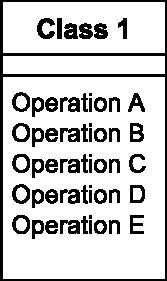
\includegraphics[width=\linewidth]{images/OriginalClassDiagram}
    \caption{origin}
    \label{fig:origin}
\end{subfigure}
\hfill
\begin{subfigure}[t]{0.2\linewidth}
    \centering
    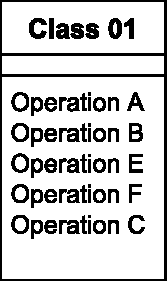
\includegraphics[width=\linewidth]{images/LeftClassDiagram}
    \caption{left}
    \label{fig:left}
\end{subfigure}
\hfill
\begin{subfigure}[t]{0.2\linewidth}
    \centering
    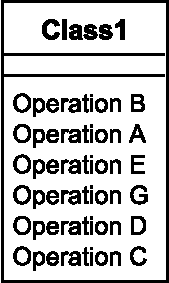
\includegraphics[width=\linewidth]{images/RightClassDiagram}
    \caption{right}
    \label{fig:right}
\end{subfigure}
\hfill
\label{fig:versions}
\caption{Different versions of a model.}
\end{figure}
\end{minipage}
\hfill
\begin{minipage}[t]{0.39\linewidth}
\begin{lstlisting}[style=eol,caption={The pseudo-formatted CBP of the model in Fig. \ref{fig:origin}.},label=lst:origincbp]
session "origin"
create x type Class
set x.name to "Math" 
create a type Operation
set a.name to "abs" 
create b type Operation
set b.name to "mean" 
create c type Operation
set c.name to "pow" 
add a to x.operations at 0
add b to x.operations at 1
add c to x.operations at 2
\end{lstlisting}
\end{minipage}

\vspace{-5pt}
\section{State-based Model Comparison}
\label{sec:model_comparison}

\vspace{-5pt}
In a collaborative modelling setting, a model is commonly developed in parallel -- thus produces different versions. Let's say that the model in Fig. \ref{fig:origin} is modified by two different modellers in parallel. The first modeller produces the model in Fig. \ref{fig:left} (the left model), and the second one yields the model in Fig. \ref{fig:right} (the right model) producing XMI files as showed in List. \ref{lst:leftxmi} and List. \ref{lst:rightxmi} respectively.

At some point, we want to compare these two models in order to identify their differences for analytics or conflicts when merging. The common approach to compare models is to create matches between the elements of both models and diff them \cite{DBLP:conf/sfm/BroschKLSWW12,emfcompare2018developer}. Generally, the matching process iterates through all the elements of the models being compared and matches them by their identifiers or through a similarity mechanism if they have none \cite{DBLP:conf/sfm/BroschKLSWW12,emfcompare2018developer}. After that, the diffing process then starts finding differences between the matched elements and all their features commonly using the Longest Common Subsequence (LCS) algorithms, e.g. \cite{DBLP:journals/algorithmica/Meyers86}. 

\vspace{-10pt}
\begin{minipage}[t]{0.49\linewidth} 
    \begin{lstlisting}[style=eol,caption={The simplified XMI of the left model in Fig. \ref{fig:left}.},label=lst:leftxmi]
    <uml:Class id="x" name="MathLib">
    <operation id="a" name="abs/>
    <operation id="d" name="sqrt"/>
    <operation id="c" name="pow"/>
    </uml:Class>
    \end{lstlisting}
\end{minipage}
\hfill
\begin{minipage}[t]{0.49\linewidth}
    \begin{lstlisting}[style=eol,caption={The simplified XMI of the right model in Fig. \ref{fig:right}.},label=lst:rightxmi]
    <uml:Class id="x" name="MathUtil">
    <operation id="b" name="mean"/>
    <operation id="c" name="pow"/>
    <operation id="a" name="abs"/>
    </uml:Class>
    \end{lstlisting}
\end{minipage}

In our example, the matching iterates through all the elements of both model using their identifiers. The matching process yields 3 matches, $m_1$ = (\textsf{x}, \textsf{x}), $m_2$ = (\textsf{a}, \textsf{a}), and $m_3$ = (\textsf{c}, \textsf{c}), and 2 umatched elements, $um_1$ = (\textsf{d},) and $um_2$ = (, \textsf{b}). The diffing process then iterates through all the matches and unmatches. Using LCS algorithm, in the first match, it identifies that both elements \textsf{x} are different in their \textsf{name} and \textsf{operations} features. 
The left \textsf{x}'s \textsf{name} is ``MathLib'' while the other \textsf{x}'s \textsf{name} is ``MathUtil'' (diff $d_1$). The \textsf{operations} features are different in their contents -- the left \textsf{operations} feature does not contain elements \textsf{b} (diff $d_2$), the left \textsf{operations} feature contains element \textsf{d} 
that does not exist in the right \textsf{operations} (diff $d_3$), and the positions of element \textsf{c} that are different in both features (diff $d_4$).

Similar to EMF Compare \cite{emfcompare2018developer}, this paper view a left model as a reference model, which means that differences are expressed as changes applied to a right model so that it equals to a reference model -- a left model. These changes share a number of common elements: \textsf{Match}, \textsf{LeftFeature}, \textsf{RightFeature} \textsf{LeftPosition}, \textsf{RightPosition}, \textsf{LeftValue}, \textsf{RightValue}, and \textsf{Kind}. \textit{Match} is the match in which diffing is performed. Since elements' identifiers are used to match elements, the identifier is used to identify the match. \textit{*Feature} and \textit{*Value} are the feature and value involved in a difference. \textsf{*Position} is the position of a value in a feature. \textit{Kind} is the type of a differences. It can be one of these types: \textsf{CHANGE}, \textsf{ADD}, \textsf{DELETE}, and \textsf{MOVE}. \textsf{CHANGE} means a pair of features -- single-valued attributes or non-containment references -- are different in their values. \textsf{ADD} indicates that a value does not exists in the right model thus it requires an addition of the value. \textsf{DELETE} is the counterpart of \textsf{ADD}. \textsf{MOVE} indicates that a matched elements are different in their locations, whether they are in the same features or cross features. 
    
Based on these definitions, we formalise the diffs identified previously as $d_n$ = [$Match_n$, $LeftFeature_n$, $RightFeature_n$, $LeftPosition_n$, $RightPosition_n$, $LeftValue_n$, $RightValue_n$, $Kind_n$]. Thus, $d_1$ =  [\textsf{x}, \textsf{name}, \textsf{name}, 0, 0, ``MathLib'', ``Mathutil'', \textsf{CHANGE}], $d_2$ = [\textsf{x}, \textsf{operations}, \textsf{operations}, -1, 0, \textsf{null}, \textsf{b}, \textsf{DELETE}], $d_3$ = [\textsf{x}, \textsf{operations}, \textsf{operations}, 1, -1, \textsf{d}, \textsf{null}, \textsf{ADD}], and $d_4$ = [\textsf{x}, \textsf{operations}, \textsf{operations}, 2, 1, \textsf{c}, \textsf{c}, \textsf{MOVE}]. Fig. \ref{fig:xmi_comparison} depicts the mapping of these diffs on the left and right models. Applying these diffs as changes to the right model will transform it into the left model.  

\vspace{-20pt}
 \begin{figure}
     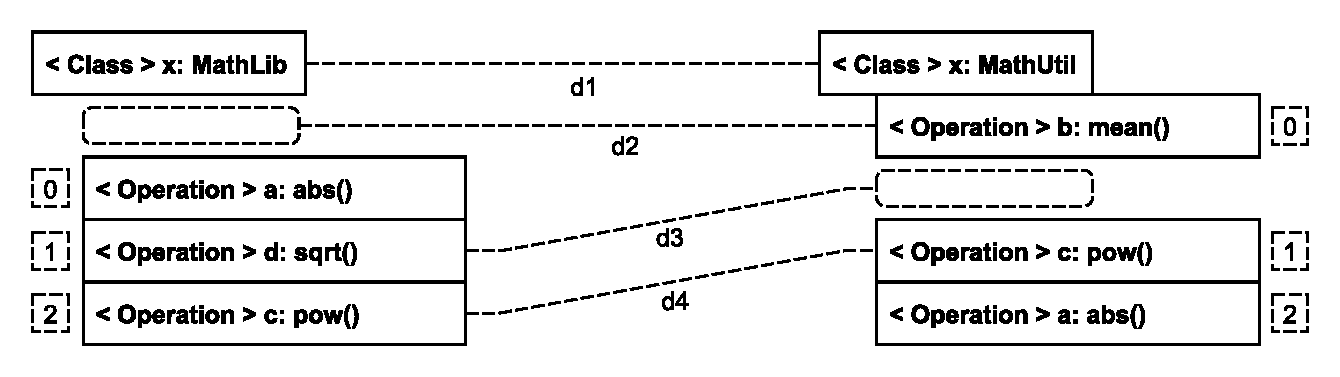
\includegraphics[width=\linewidth]{images/XmiComparison}
     \caption{A model comparison of the left and right models in Listings \ref{lst:leftxmi} and \ref{lst:rightxmi}.}
     \label{fig:xmi_comparison}
 \end{figure}
 
\vspace{-20pt}
\section{Change-based Approach for Comparing Models}
\label{sec:change_based_approach_for_comparing_models}

\vspace{-20pt}
 \begin{figure}
    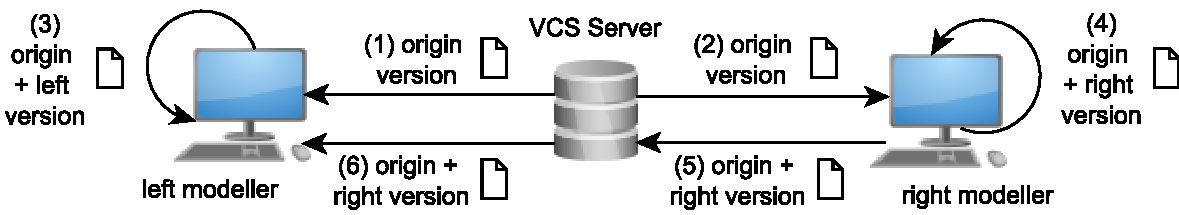
\includegraphics[width=\linewidth]{images/VCS}
    \caption{A case of the use of CBP in a collaborative modelling.}
    \label{fig:vcs}
\end{figure}

\vspace{-10pt}
In the context of collaborative modelling using CBP, let's say that the file of the CBP in \ref{lst:origincbp} already existed in a text-based Version Control System (VCS) server (Fig. \ref{fig:vcs}). Both modellers checkout the original CBP (steps 1 and 2) and modify it (steps 3 and 4). Changes made by the left and right modellers will be appended to the original CBP producing two different CBP representation as displayed in Listings \ref{lst:leftcbp} and \ref{lst:rightcbp}\footnote{Both CBPs only present the changes after the last line of the original version (start from line 19). In implementation, the changes are appended to the original version.} -- capturing different courses of modification made by the modellers. The right developer then commits her work (original + right version) to the VCS. Since there is no new commit on the VCS, the commit process is straightforward (step 5). The left developer then decide to also commit his work (original + left version) to the VCS, thus his machine downloads the current version from the server (step 6). However, since the original version has been updated since his last checkout, he has to perform a model comparison to check the differences, and possibly conflicts, between his version (original + left version) and the updated original version (original + right version). 

\begin{minipage}[t]{0.49\linewidth}    
\begin{lstlisting}[firstnumber=13,style=eol,caption={The CBP of the model in Fig. \ref{fig:left} (left version).},label=lst:leftcbp]
session "left"
set x.name from "Math" to "MathLib"
create d type Operation
set d.name to "sqrt"
add d to x.operations at 1
remove b in x.operations at 2
delete b
\end{lstlisting}
\end{minipage}
\hfill
\begin{minipage}[t]{0.49\linewidth}
\begin{lstlisting}[firstnumber=13,style=eol,caption={The CBP of the model in Fig. \ref{fig:right} (right version).},label=lst:rightcbp]
session "right"
move a in x.operations from 0 to 2
set x.name from "Math" to "MathUtil"
\end{lstlisting}
\end{minipage}

Since both modellers work using CBP, we can exploit the persistence to improve the previous model comparison. For example, we do not need to visit, match, and differentiate both elements \textsf{c} in the running example as it is not affected by the recent changes in both CBPs; only the affected features by the recent changes to be compared -- not all features. 

In performing comparison, our approach has three phases: event loading, element tree construction, and diff computation. These phases are represented as methods \textsf{loadEvents}, \textsf{contructElementTree}, and \textsf{computeDifferences} methods in class \textsf{CBPComparison} in Fig. \ref{fig:approach_class_diagram}. 

\vspace{-10pt}
\begin{figure}
    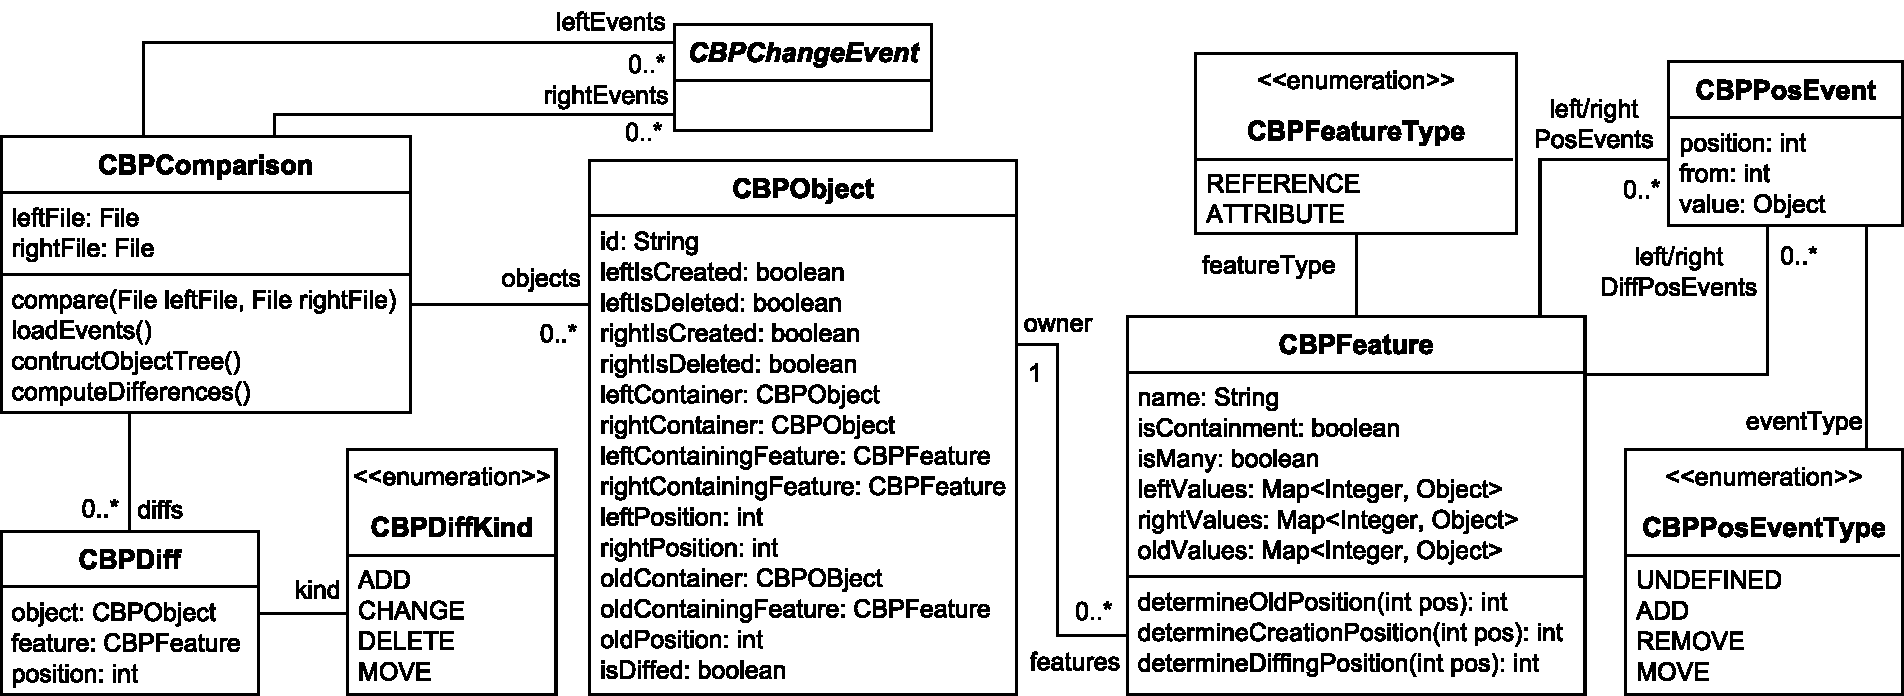
\includegraphics[width=\linewidth]{images/TreeClassDiagram}
    \caption{A class diagram showing the core components of the change-based approach to optimise model comparison.}
    \label{fig:approach_class_diagram}
\end{figure}

\vspace{-20pt}
\subsection{Event Loading}
\label{sec:event_loading}
In the event loading, our implementation loads two supplied CBP files into memory as change-event instances of the class \textsf{ChangeEvent} in Fig. \ref{fig:approach_class_diagram}. Not all lines are converted into change events. Only lines starting from the position where the two files are different are loaded as change-events. In this case, lines 1-12 in List. \ref{lst:origincbp} are not loaded. Only lines starting from line 13 in Listings \ref{lst:leftcbp} and \ref{lst:rightcbp} are loaded, yielding two lists -- left and right -- of change events. 

\subsection{Element Tree Construction}
\label{sec:tree_construction}
An element tree is similar to the list of matches in the previous model comparison except that, some of the differences, it has several flags (e.g.\textsf{*isCreated}, \textsf{*isDeleted} in class \textsf{Element}, Fig. \ref{fig:approach_class_diagram}), it uses Map data structure instead of List (class \textsf{Feature}, Fig. \ref{fig:approach_class_diagram}) to represent multi-valued features of the left and right models, and the presence of attribute \textsf{oldValues} to hold the original values of features. These specific features are useful to determine differences in the diff computation phase.

\IncMargin{1.5em}
\begin{algorithm}[H]
    \begin{footnotesize}
        \SetKwInOut{Input}{input}
        \SetKwInOut{Output}{output}
        \Input{a list of ChangeEvent $events$}
        \Input{an enumeration of Side $side$}
        \Input{an instance of ElementTree $elementTree$}
        \Output{an instance of ElementTree $elementTree$}
        \SetKwBlock{Beginn}{beginn}{ende}
        \Begin{
            \ForEach{$event$ in $events$}{
                $targetElement$ $\leftarrow$ getOrCreateNewTargetElement($event$, $elementTree$)\;
                $feature$ $\leftarrow$ getOrCreateNewFeature($event$, $targetElement$)\;
                $value$ $\leftarrow$ getValue($event$)\;
                $previousValue$ $\leftarrow$ getPreviousValue($event$)\;
                $position$ $\leftarrow$ getPosition($event$)\;
                $previousPosition$ $\leftarrow$ getPreviousPosition($event$)\;
                $featureEventList$ $\leftarrow$ getFeatureEventList($feature$, $side$)\;
                
                \BlankLine
                \tcp{put all values to their proper positions}
                updateTree($targetElement$, $feature$, $value$, $position$, $side$)\;
                $oldPosition$ $\leftarrow$ calculateOldPosition($featureEventList$, $previousPosition$, $side$)\;
                \If{\Not isCreated($value$, $side$) \And isOldValueSet($feature$, $previousValue$, $previousPosition$, $side$) \Is false} {
                    setOldValue($feature$, $previousValue$, $oldPosition$, $side$)\;
                    $oppositeFeatureEventList$ $\leftarrow$ getOppositeFeatureEventList($feature$, $side$)\;
                    $oppositePosition$ $\leftarrow$ calculateOppositePosition($oppositeFeatureEventList$, $oldPosition$, $side$)\;
                    \If{isOppositeSideValueSet($feature$, $value$, $oppositePosition$, $side$) is False} {
                        setOppositeSideValue($feature$, $value$, $oppositePosition$, $side$)\;
                    }
                }   
                
                addEventToFeatureEventList($event$, $featureEventList$)\;
                
            }
        \Return{$elementTree$}\;
        }
    \end{footnotesize}
    \caption{Algorithm to construct an element tree from events.}
    \label{alg:element_tree}
\end{algorithm}
\DecMargin{1.5em}

The construction of the element tree execute the following outline. First, an empty element tree is created. After that, the process iterates through all left model's change events and uses the information contained in the change events to construct the partial states of the left, original, and right models. After finish with the left change events, the process then iterates the change events of the right model. Similarly, using the information available in the right change events, the process updates the partial states of the right, original model, and left models. 

The element three construction conforms to the Alg. \ref{alg:element_tree}. The selection of side which side, left or right change events, that is executed first depends on the \textsf{Side} enumeration value -- \textsf{left} or \textsf{right} -- passed through the parameter \textsf{side} (the second input parameter). The algorithm also receives an input of the change events \textsf{events} that are to be iterated and the element tree \textsf{elementTree} that has been instantiated before, and then return the \textsf{elementTree} as an output after updating it.

For each \textsf{event} in the \textsf{events}, we collects information needed to build up the element tree (lines 3-9), such as \textsf{targetElement}, \textsf{feature}, \textsf{value}, \textsf{previousValue}, \textsf{position}, and \textsf{previousPosition}. The \textsf{targetElement} is the element modified by a change event (e.g. \textsf{x} and \textsf{d} in List. \ref{lst:leftcbp}). This \textsf{targetElement} -- an instance of class Element in Fig. \ref{fig:approach_class_diagram} -- is retrieved from the \textsf{elementTree} if it already exists, otherwise a new one is created and added to the \textsf{elementTree} (line 3). In this step also we set the flags \textsf{*IsCreated} and \textsf{*IsDeleted} of the element in Fig. \ref{fig:approach_class_diagram}. For example, if the type of the event is \textsf{create} then \textsf{*IsCreated} is set to \textsf{true}. The \textsf{feature} -- an instance of class Feature in Fig. \ref{fig:approach_class_diagram} -- represents the target element's feature (e.g. \textsf{name} and \textsf{operations} in List. \ref{lst:leftcbp}) modified by a change event. It is  retrieved from the \textsf{targetElement}'s feature list, and a new one is created and added to the \textsf{targetElement}'s feature list, if it has not existed yet (line 5). 

The \textsf{value} is the value assigned to the feature in a change event (line 5, Alg. \ref{alg:element_tree}). The \textsf{value} can be type of \textsf{Element} (e.g. elements \textsf{b} and  \textsf{d}, lines 17-18, List. \ref{lst:leftcbp}) or primitive (e.g. the String ``MathLib'' at line 14 in the List. \ref{lst:leftcbp}). The \textsf{previousValue} is similar to the \textsf{value} except that it represents the previous value of the modified feature (line 6, Alg. \ref{alg:element_tree}). The \textsf{previousValue} is not defined if there is no previous value has been assigned. If the type of \textsf{value} and \textsf{previousValue} is \textsf{Element}, the elements that they represents are retrieved from the \textsf{elementTree} otherwise new instances are created if they are contained yet in the \textsf{elementTree}. Not every change event has \textsf{value}, particularly event with type \textsf{add} or \textsf{delete} as it only modifies a target element not the element's feature.

The \textsf{position} is the position assigned by a change event to a value in a feature, while \textsf{previousPosition} is the previous position of the value (lines 7-8, Alg. \ref{alg:element_tree}). In one change event, we can get both \textsf{position} and \textsf{previousPosition} or only one of them depends on the type of the change event. For example, we can only obtain that the \textsf{position} of \textsf{d} is 1 (line 17 in in the List. \ref{lst:leftcbp}) as the change event type is \textsf{add}. In \textsf{remove} change event, we can only get the \textsf{previousPosition} of \textsf{b}, that is 2 (line 17 in in the List. \ref{lst:leftcbp}), as the element does not exists anymore in the left model. We can obtain both of them only in a \textsf{move} change event as an element is moved from a previous position to a new one (line 14 in in the List. \ref{lst:rightcbp}). For a single-valued feature, the \textsf{position} and \textsf{previousPosition} are always 0 as the feature can only contains a value. 

At line 9, we retrieve the \textsf{featureEventList} from the \textsf{feature} to be added later with the current \textsf{event} (line 19). The \textsf{featureEventList} is a list -- a history -- of change events that have been processed specific to the \textsf{feature} on the defined \textsf{side}. Using the obtained \textsf{targetElement}, \textsf{feature}, \textsf{value}, and \textsf{position}, the process then updates the state of the \textsf{elementTree} on the selected \textsf{side} (line 10). After that, it calculates back the original position of a value using the \textsf{featureEventList} and \textsf{previousPosition} (line 11). If the value at \textsf{oldPosition} in the \textsf{feature} has not been set, then the algorithm sets the \textsf{feature} with the \textsf{previousValue} at the \textsf{oldPosition} in the partial state of the original model (lines 12-13). At lines 14-18, the algorithm also does the same thing to the opposite side -- if the current \textsf{side} is \textsf{left} then it is \textsf{right}.  

To better understand how the algorithm works, we explain its execution using both change events in the Listings \ref{lst:leftcbp} and \ref{lst:rightcbp}. We start from the left change events. 

\begin{wrapfigure}[19]{r}{0.5\textwidth}
    \vspace{-20pt}
    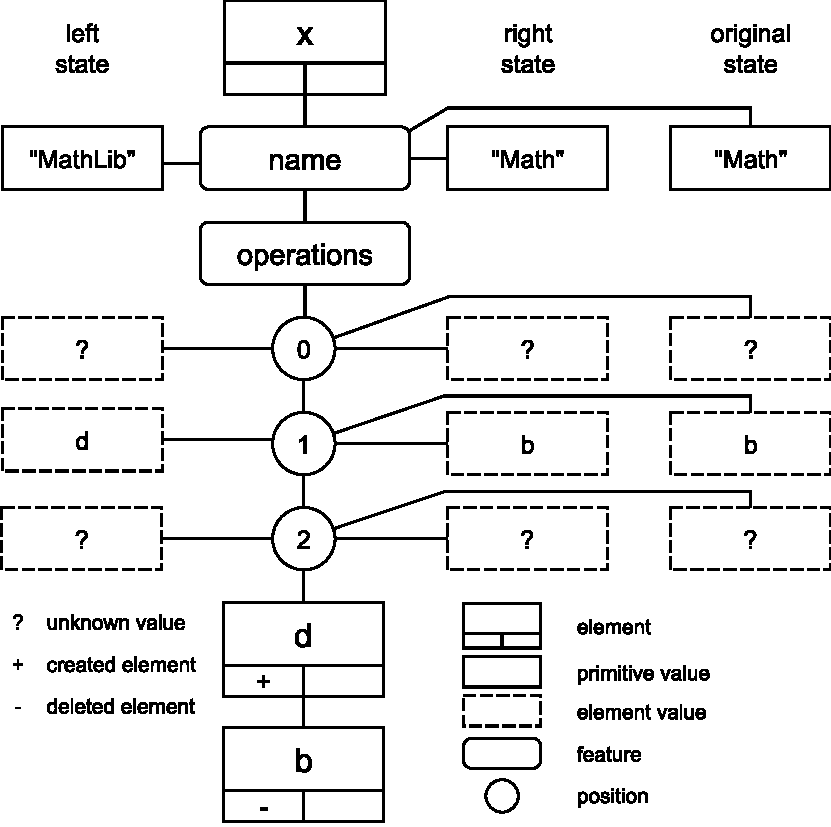
\includegraphics[width=\linewidth]{images/LeftElementTreeDiagram}
    \caption{A class diagram showing the core components of the change-based approach to optimise model comparison.}
    \label{fig:left_element_tree_diagram}
\end{wrapfigure}

\vspace{-10pt}
\subsubsection{Left Side.}\label{sec:left_side} In List. \ref{lst:leftcbp}, the first event is a \textsf{session} event (line 13). \textsf{Session} event indicates that its following events -- until the next session event or end of file -- are one batch of changes when they were persisted into a change-based persistence file. This event is not significant for model comparison, thus skipped. 

In the next event, \texttt{\small \textbf{set} x.name \textbf{from} "Math" \textbf{to} "MathLib"} (line 14), we can identify that there is an element with id \textsf{x} that has been existed from the original model. It has a feature \textsf{name} with a value ``Math'' in the original model and has been changed to ``MathLib'' in the left model. Since the element \textsf{x} has not existed in the $elementThree$, we create its instance of \textsf{Element} and also its feature \textsf{name}. We set the value of the feature \textsf{name} to ``MathLib'' and also set it to ``Math'' in the partial state of the original model -- it has not been set before. As the same feature in the right side also has not been set, we set it to ``Math'' as well.          

In the event at line 15, \texttt{\small \textbf{create} d \textbf{type} Operation}, we can indentify that there an element with id \textsf{d} has been created. We also update the \textsf{elementTree} to include this element and set the element's flag \textsf{leftIsCreated} to \textsf{true}. In the event at line 16, \texttt{\small \textbf{set} d.name \textbf{to} "sqrt"}, we can identify that element \textsf{d}'s feature \textsf{name} has been set to ``sqrt''. Thus, we update the \textsf{d}'s feature \textsf{name} in the \textsf{elementTree}. From the event at line 1, \texttt{\small \textbf{add} d \textbf{to} x.operations \textbf{at} 1}, we can deduce that element \textsf{d} is added to position 1 in the element \textsf{x}'s feature \textsf{operations}. Thus, we assign \textsf{d} to element \textsf{x}'s feature \textsf{operations} at position 1 in the \textsf{elementTree}. As \textsf{d} is a new element that only exists in the left model, we do not update changes of this element to the original and right models. 

From the event at line 18, \texttt{\small \textbf{remove} b \textbf{in} x.operations \textbf{at} 2}, we can identify that there is element \textsf{b} in the original model, but it is deleted in the left model. The position of element \textsf{b} in the original model is calculated by comparing its position to the previous change events of feature that contains the element \textsf{b}.  


%session "left"
%set x.name from "Math" to "MathLib"
%create d type Operation
%set d.name to "sqrt"
%add d to x.operations at 1
%remove b in x.operations at 2

At line 2, the event  , there is an element with id \textsf{x}. The element has a feature \textsf{name} with values ``Math'' in its original model and ``MathLib'' in its eventual left version. Also, from the event \textsf{\small \textbf{move} a \textbf{in} x.operations \textbf{from} 0 \textbf{to} 2}, there is an element with id \textsf{a}, and the element is contained in in the feature \textsf{operations} of element \textsf{x}. 




\subsubsection{Right Side.} 
\label{sec:right_side}

\begin{wrapfigure}[21]{r}{0.5\textwidth}
    \vspace{-20pt}
    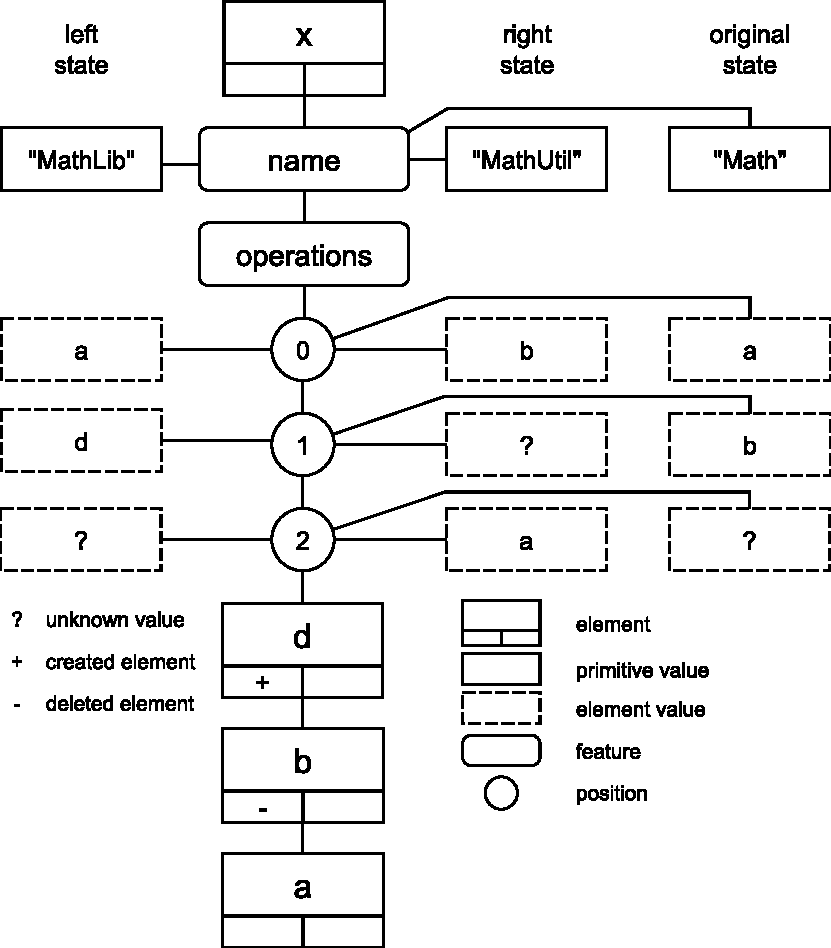
\includegraphics[width=\linewidth]{images/RightElementTreeDiagram}
    \caption{A class diagram showing the core components of the change-based approach to optimise model comparison.}
    \label{fig:right_element_tree_diagram}
\end{wrapfigure}

The iteration continues to the right CBP. The line 1 is skipped since it is a session event.  At line 2, a CBP object with id $ob$ and CBP feature $name$ is created. The values of CBP feature $name$ are also set so that it has $rightValues$[0] = ``Operation BB'', $oldValues$[0] = ``Operation B'', and $leftValues$[0] = ``Operation B''. 

\subsection{Diff Computation}
\label{sec:diff_computation}
Our approach determines the differences between the two models by iterating through the element tree in Table \ref{table:right_object_tree} and making use of the states of values and $^*IsCreated$ and $^*IsDeleted$ flags. At CBP object $c$, the values of CBP feature $name$ are different between the left and the right sides. Thus, to make the right value equals to the left value, the value has to be change from ``Class X'' to ``Class 01''. Thus, we can determine that the first diff is $d_1^\prime$ = [\textsf{c}, \textsf{name}, ``Change 01'', \textsf{CHANGE}], which as are equal to $d_1$ that is defined in Sect. \ref{sec:change-based_persistence}.

\IncMargin{1.5em}
\begin{algorithm}[H]
    \begin{footnotesize}
        \SetKwInOut{Input}{input}
        \SetKwInOut{Output}{output}
        \Input{an instance of ElementTree $elementTree$}
        \Begin{
            $diffList$ $\leftarrow$  DiffList()\;
            \ForEach{$element$ in $elementTree$}{
                \ForEach{$feature$ in getFeatures($element$)}{
                    \ForEach{$position$ in getPositions($feature$)}{
                        $leftValue$ $\leftarrow$ getLeftValue($feature$, $position$)\;
                        $rightValue$ $\leftarrow$ getRightValue($feature$, $position$)\;
                        \BlankLine
                        \tcp{rules starts from here}
                        \uIf{isReference($feature$)}{
                            \tcp{. . .}
                            \If{isMultiValued($feature$)}{
                                \If{\Not isNull($leftValue$)}{
                                    \uIf{isLeftCreated($leftValue$) \And\Not isLeftDeleted($leftValue$) \And\Not isRightCreated($leftValue$) \And\Not isRightCreated($leftValue$)}{
                                       $diff$ $\leftarrow$ createDiff($element$, $feature$, $value$, $position$, DiffType.ADD)\;
                                       addToDiffList($diff$,$diffList$)\;
                                    }
                                }
                            }
                            \tcp{. . .}
                        }\ElseIf{isAttribute($feature$)}{
                            \tcp{. . .}
                            \If{isSingleValued($feature$)}{
                                \If{\Not isNull($leftValue$) \And \Not isNull($rightValue$)}{
                                    $diff$ $\leftarrow$ createDiff($element$, $feature$, $leftValue$, $position$, DiffType.CHANGE)\;
                                    addToDiffList($diff$, $diffList$)\;
                                }
                            }
                            \tcp{. . .}
                        }
                    }
                }
            }
            \Return{$diffList$}\;
        }
    \end{footnotesize}
    \caption{Algorithm to determine differences.}
    \label{alg:diff_calculation}
\end{algorithm}
\DecMargin{1.5em}

At position 0 in CBP feature $operations$ of CBP object $c$, the values are different between the left and the right sides -- '??' and $ob$ respectively. Since the left value is undefined, we check the flags of $ob$. All flags $^*IsCreated$ and $^*IsDeleted$ are in the $false$ state, which means element \textsf{ob} has been existed since the original version -- it has never been created or deleted in recent changes. Thus, the only possible type of change is move. Thus by checking the attributes $leftPosition$ and $rightPosition$ in class \textsf{Element} (in Fig. \ref{fig:approach_class_diagram}), the positions of element \textbf{ob} are different between the left and right sides -- at positions 1 and 0 respectively. Therefore, we can decide that the second diff is $d_2^\prime$ = [\textsf{c}, \textsf{operations}, \textsf{ob}, \textsf{MOVE}]. The flag \textit{isDiffed} of CBP object $ob$ is set to $true$ so that it can be skipped when processing values at position 1 -- the next position.  

The values at position 2 in CBP object $c$'s $operations$ CBP feature are equal. Therefore, there is no diff at this position. At position 3, the values are different -- $of$ and $og$. When checking the $^*IsCreated$ and $^*IsDeleted$ flags, we can identify that both $of$ and $og$ have been separately created in the left and right recent changes respectively -- both has their $^*IsCreated$ flags are set to $true$. Thus, we can infer that $of$ and $og$ have been added to the position. To make the right model equals to the left model, element \textsf{of} should be added to the right side, and element \textsf{og} should be deleted. Thus, we can determine the third diff as $d_3^\prime$ = [\textsf{c}, \textsf{operations}, \textsf{of}, \textsf{ADD}] and the fourth diff as $d_4^\prime$ = [\textsf{c}, \textsf{operations}, \textsf{og}, \textsf{DELETE}].

At position 4 in CBP feature $operations$ of CBP object $c$, the values are not equal. When checking their $^*IsCreated$ and $^*IsDeleted$ flags, we can infer that $oc$ has been existed since the original version -- all its $^*IsCreated$ and $^*IsDeleted$ flags are $false$ -- and $od$ is deleted from the left model -- its $leftIsCreated$ flag is $true$. The $leftPosition$ and $rightPosition$ of $oc$ are also checked and their values are different -- 4 and 5 respectively. Thus, to make the right model equals to the left model, element \textsf{oc} should be moved from 5 to 4, element \textsf{od} should be deleted. Therefore, we can formulate  that the fifth diff is $d_5^\prime$ = [\textsf{c}, \textsf{operations}, \textsf{oc}, \textsf{MOVE}] and the sixth diff is $d_6^\prime$ = [\textsf{c}, \textsf{operations}, \textsf{od}, \textsf{DELETE}]. 

However, due to the design of features in Ecore/EMF metamodel, deleting an element from a feature shifts all the positions of the following elements one step downward. So it is not necessary to define $d_5^\prime$ as the position of \textsf{oc} is automatically stepped down from 5 to 4 if the \textit{deletion} ($d_6^\prime$) is executed first. To accommodate this, \textit{deletion} is given priority over \textit{move}. 

More explanation will be added here.

\section{Evaluation Method}
\label{sec:evaluation}

In order to evaluate the performance of the change-based approach on model comparison, we have evaluated it against the traditional state-based approach as the benchmark. We choose EMF Compare \cite{emfcompare2018developer,eclipse2017compare} as the tool to perform the state-based comparison since it is a common tool to compare EMF-based models. Since we could not find any existing large models persisted in change-based format to be used as the dataset for our experiments, we reverse-engineered a large model -- it confirms the Java metamodel \cite{eclipse2018modiscojava} -- from the Epsilon project \cite{eclipse2018epsilongit,eclipse2017epsilon}. The model consists of more than 1.6 million elements with size of 224 MBs persisted in XMI format. 

We cloned the original model to produce two new -- left and right -- models and perform random changes -- random operations (e.g. add, remove, move, set) with random elements, features, positions, and values -- to both models to create differences between them. Since we wanted the change of total elements did not affect our measurement, the probabilities of executing \textit{add} and \textit{remove} operations were made equal, thus the total number of elements can be kept constant, and the modification can still include both operations. We made 1.1 million changes to each model which generated more than 1.1 millions events (one operation can generate more than one event, e.g. a \textit{move} between features generates \textit{remove} and \textit{add} events). Events generated by the changes were persisted in change-based format (to be used later in change-based model comparison). After every 50 thousand changes, we also persisted the last state of the models in state-based format (to be used later in state-based model comparison) and then performed the change-based and state-based model comparison and measured their comparison time and memory footprint, thus produced 22 records of measurement. 

Since the change-based and state-based approaches can produce different differences, in order to evaluate the correctness of the change-based approach, we reconciled all the differences by performing all-left-to-right merging -- making the right model identical to the left model -- based on the identified differences. If the all-left-to-right merging of change-based approach produces a model that is identical to the model produced by the all-left-to-right merging of the state-based approach then it can be said that differences identified by the change-based approach are correct. We performed this correctness checking at every time the measurement mentioned above was executed.

\section{Result and Discussion}
\label{sec:discussion}

\begin{figure}[ht]
    \centering
    \begin{subfigure}[t]{0.495\linewidth}
        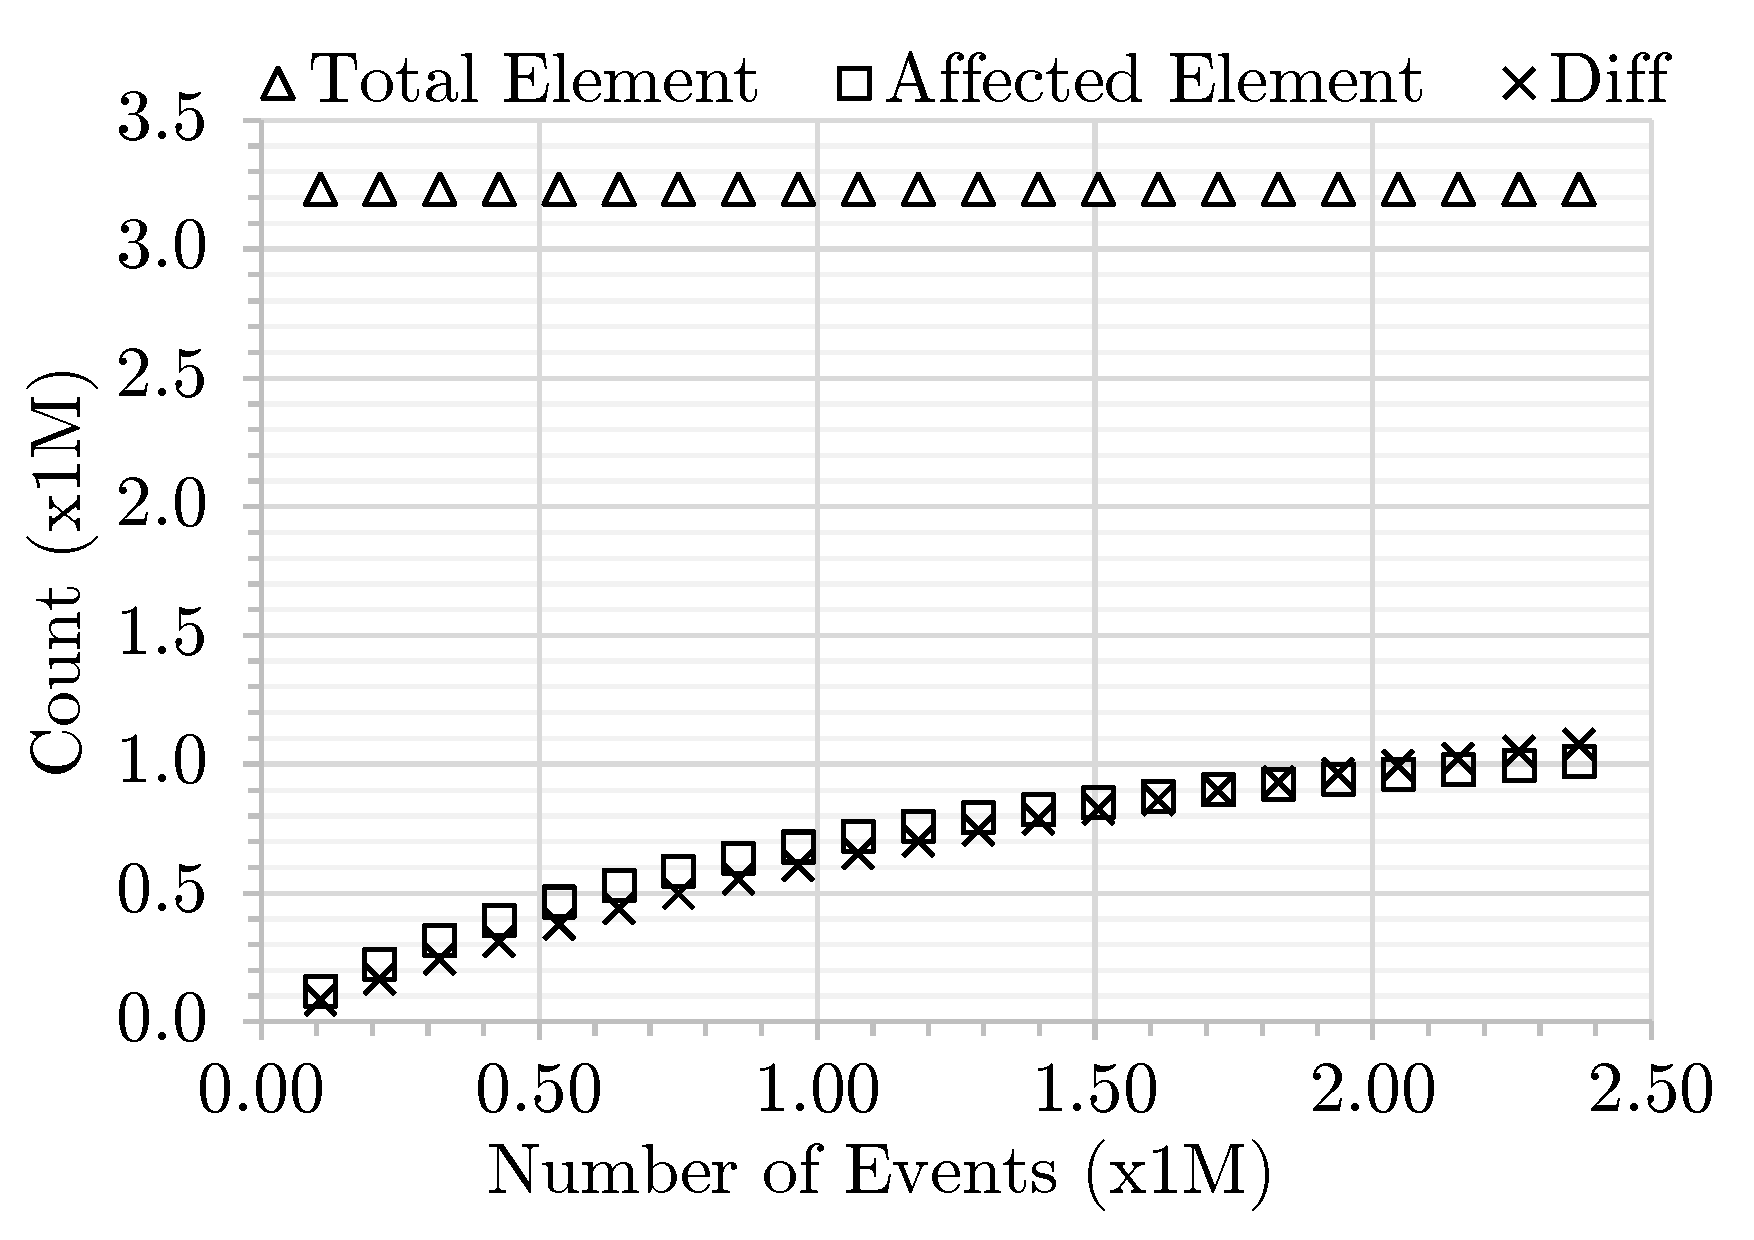
\includegraphics[width=\linewidth]{images/ModificationCourse}
        \caption{total elements, affected elements, and diffs}
        \label{fig:modification_course}
    \end{subfigure}
    \hfill
    \begin{subfigure}[t]{0.495\linewidth}
        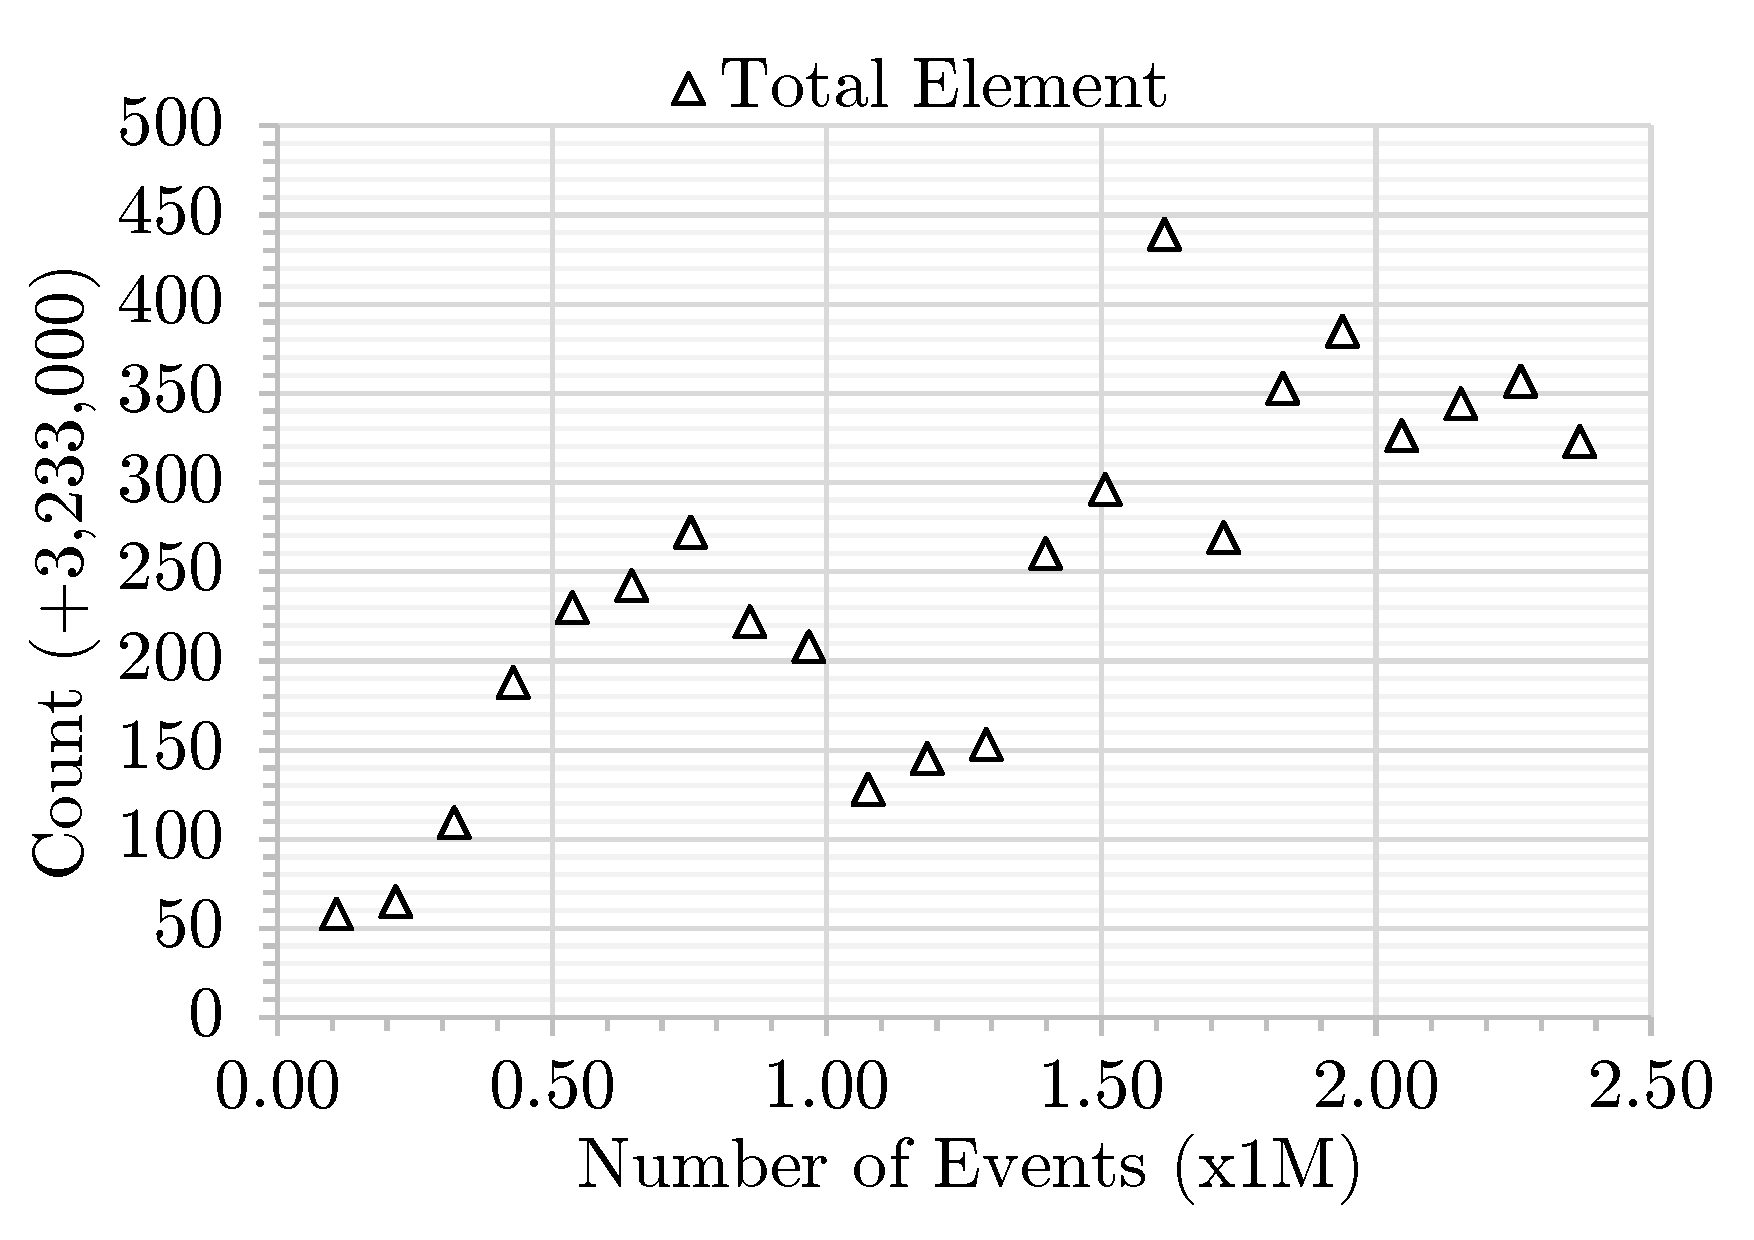
\includegraphics[width=\linewidth]{images/ModelSize}
        \caption{zoom-in view of total elements in Fig. \ref{fig:modification_course}}
        \label{fig:model_size}
    \end{subfigure}
    \caption{Changes on models along the artifical modification.}
    \label{fig:modification_model_size}
\end{figure}

Fig. \ref{fig:modification_model_size} depicts the the modification course stated in the Section \ref{sec:evaluation}. The increase of events correlates positively to the number of affected elements and differences. As the number of events inclines, the probability of changes that modify already-affected elements or features also gets higher. Thus, some changes might not contribute to the addition of new affected elements or differences -- more changes are required to add or create new elements or differences. In consequence, both grows in logarithmic manner as can be seen in Fig. \ref{fig:modification_course}. As designed in the the Section \ref{sec:evaluation}, the number of total elements of both models is almost constant. The total of elements of both models does change but in the order of hundreds (in constrast, both models have more than 3.2 millions in total). Fig. \ref{fig:model_size} depicts the zoom-in view of the total elements in Fig. \ref{fig:modification_course}.

\begin{figure}[ht]
    \centering
    \begin{subfigure}[t]{0.495\linewidth}
        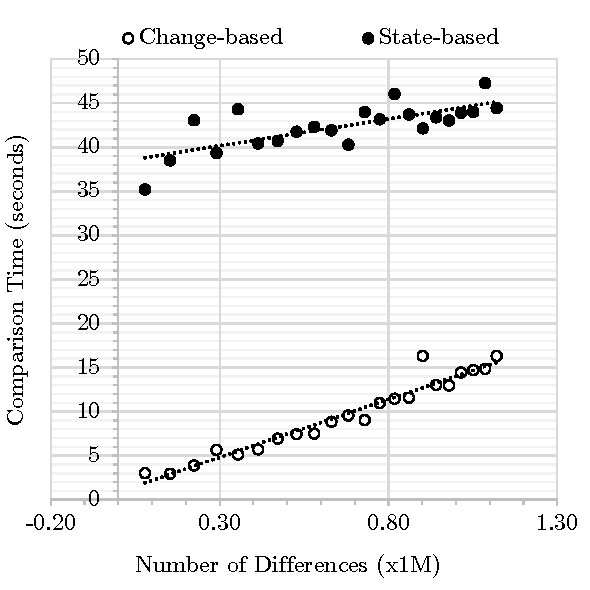
\includegraphics[width=\linewidth]{images/Time-Diffs}
        \caption{execution time}
        \label{fig:time_diffs}
    \end{subfigure}
    \hfill
    \begin{subfigure}[t]{0.495\linewidth}
        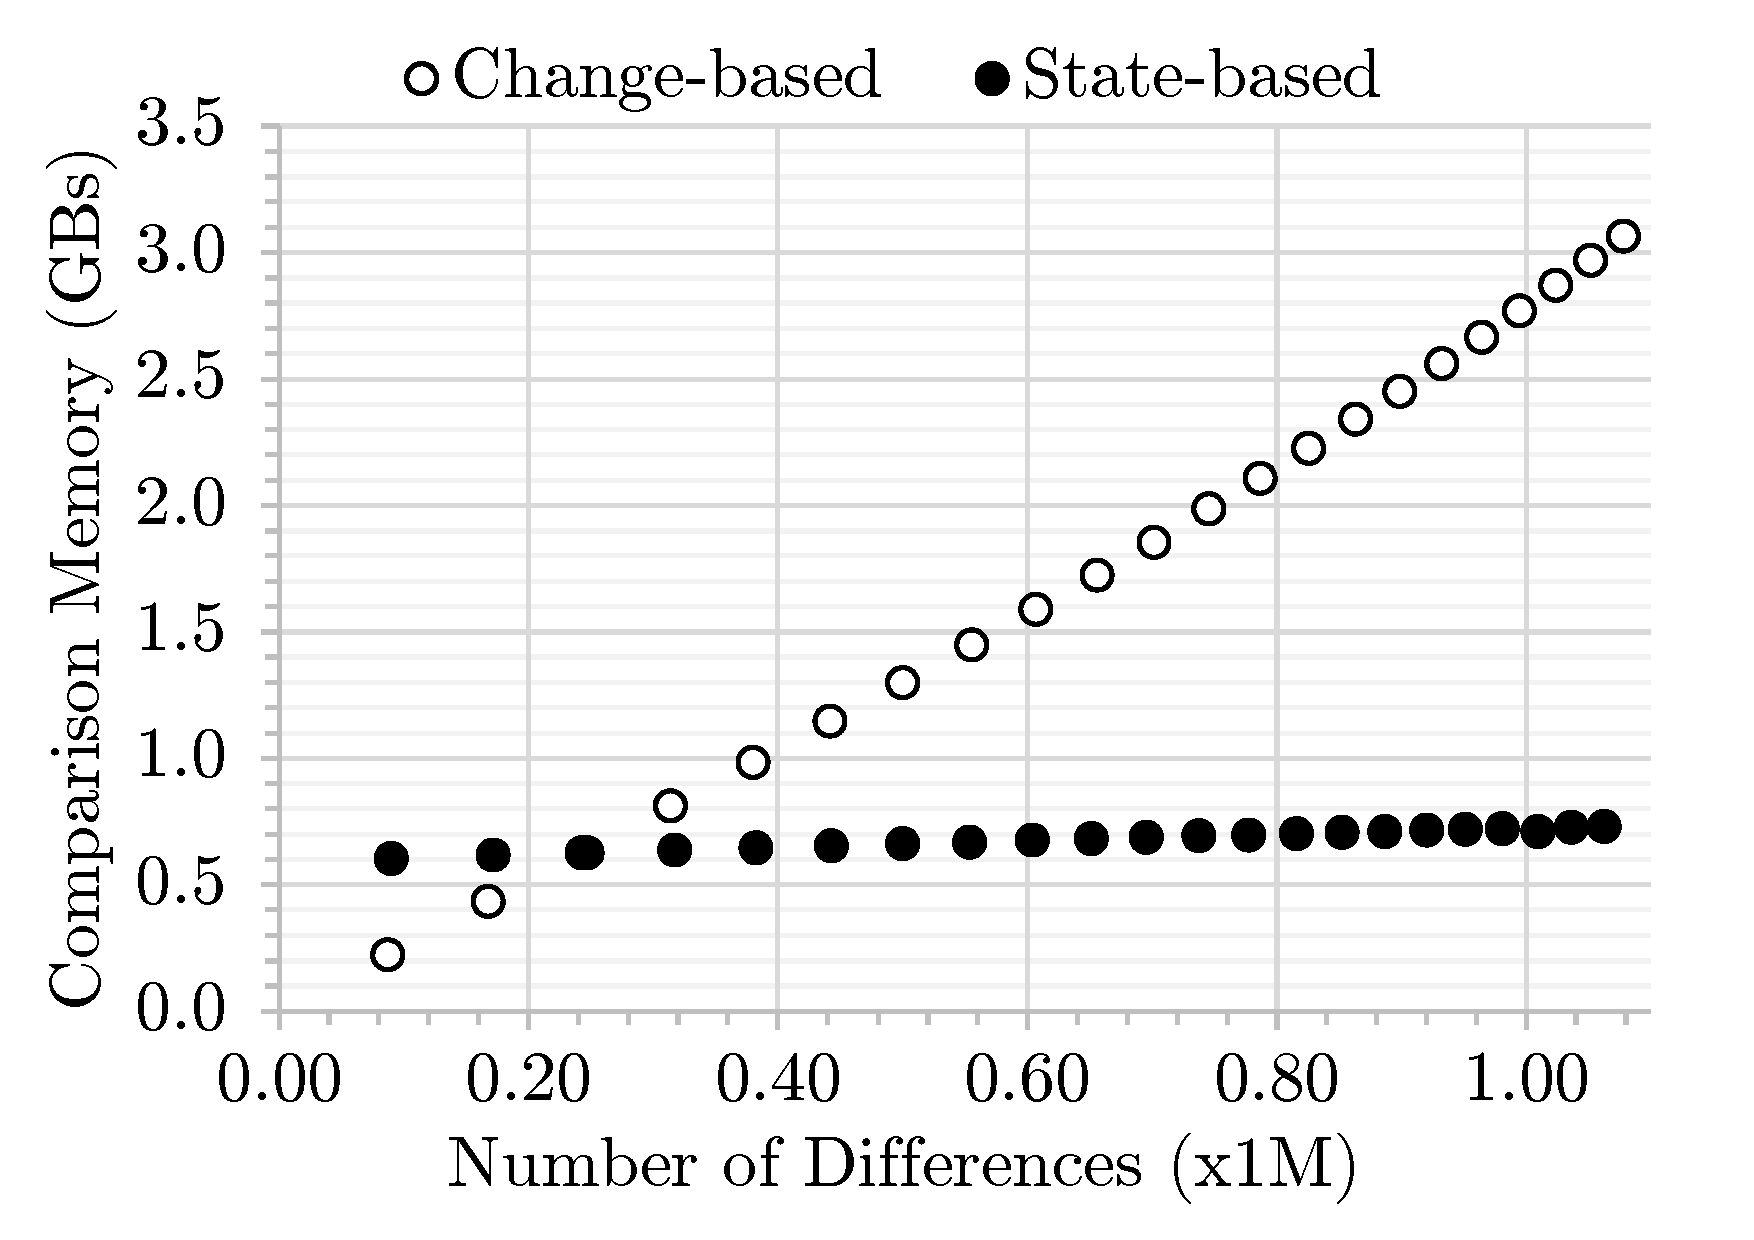
\includegraphics[width=\linewidth]{images/Memory-Diffs}
        \caption{memory footprint}
        \label{fig:memory_diffs}
    \end{subfigure}
    \caption{Change-based vs. state-based model comparison as differences increase.}
    \label{fig:change_vs_state}
\end{figure}

Figures \ref{fig:time_diffs} and \ref{fig:memory_diffs} shows the execution time and memory footprint of the change-based and state-based comparison to contrast their performance. We can notice that the change-based comparison outperforms the state-based comparison in terms of execution time. The change-based approach only requires 5 seconds compared to the state-based approach that takes 66 seconds to identify around 90,000 differences (see the first circles). However, as the number of differences grows -- which also indicates increase on events, a growing number of events also have to loaded also into memory for the construction of the element three thus slows down the comparison. Fig. \ref{fig:time_changediff_detail} breaks down the comparison time in detail. It exhibits that the event loading time is the dominant contributor to the slowdown compared to the element tree's construction time and diffing time -- the diffing time is the weakest contributor. 

\begin{figure}[ht]
    \centering
    \begin{subfigure}[t]{0.495\linewidth}
        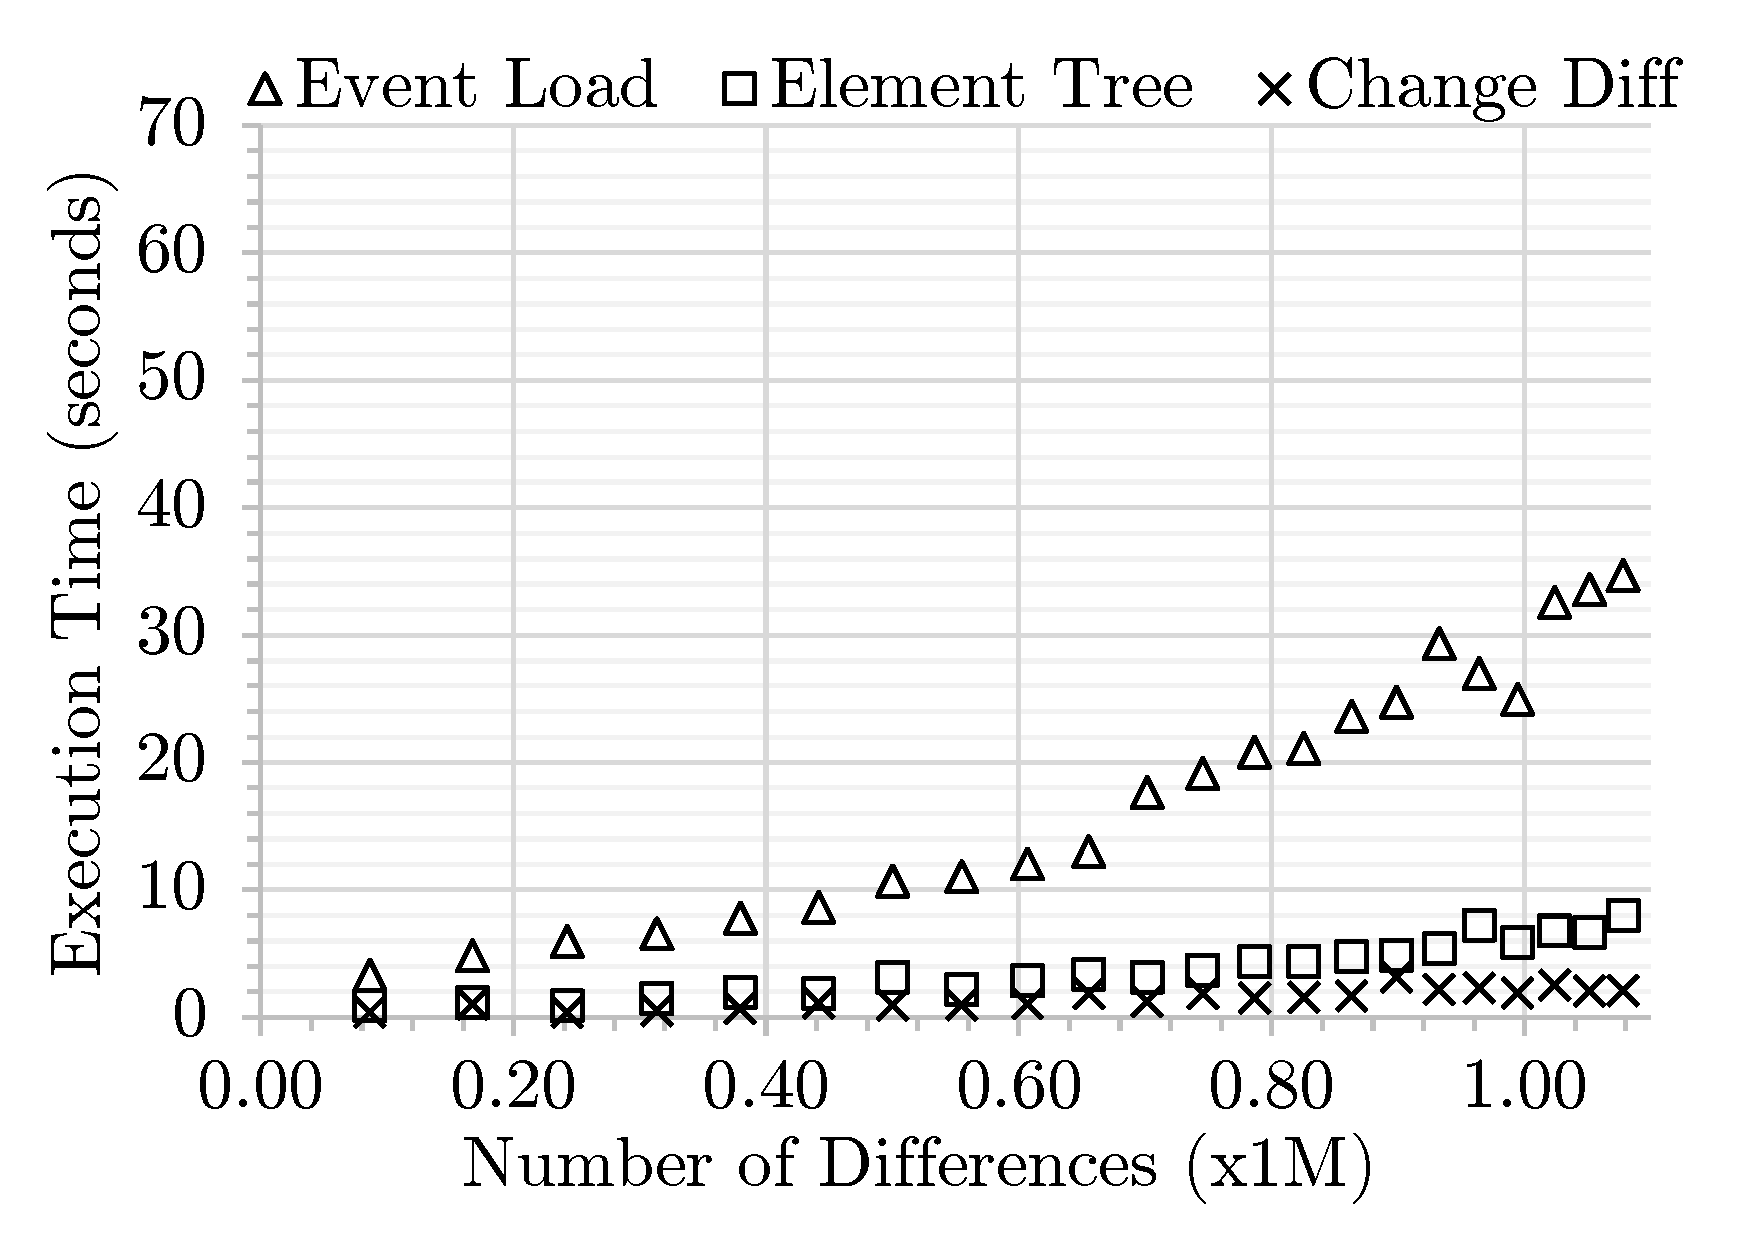
\includegraphics[width=\linewidth]{images/Time-ChangeDiff-Detail}
        \caption{change-based execution time}
        \label{fig:time_changediff_detail}
    \end{subfigure}
    \hfill
    \begin{subfigure}[t]{0.495\linewidth}
        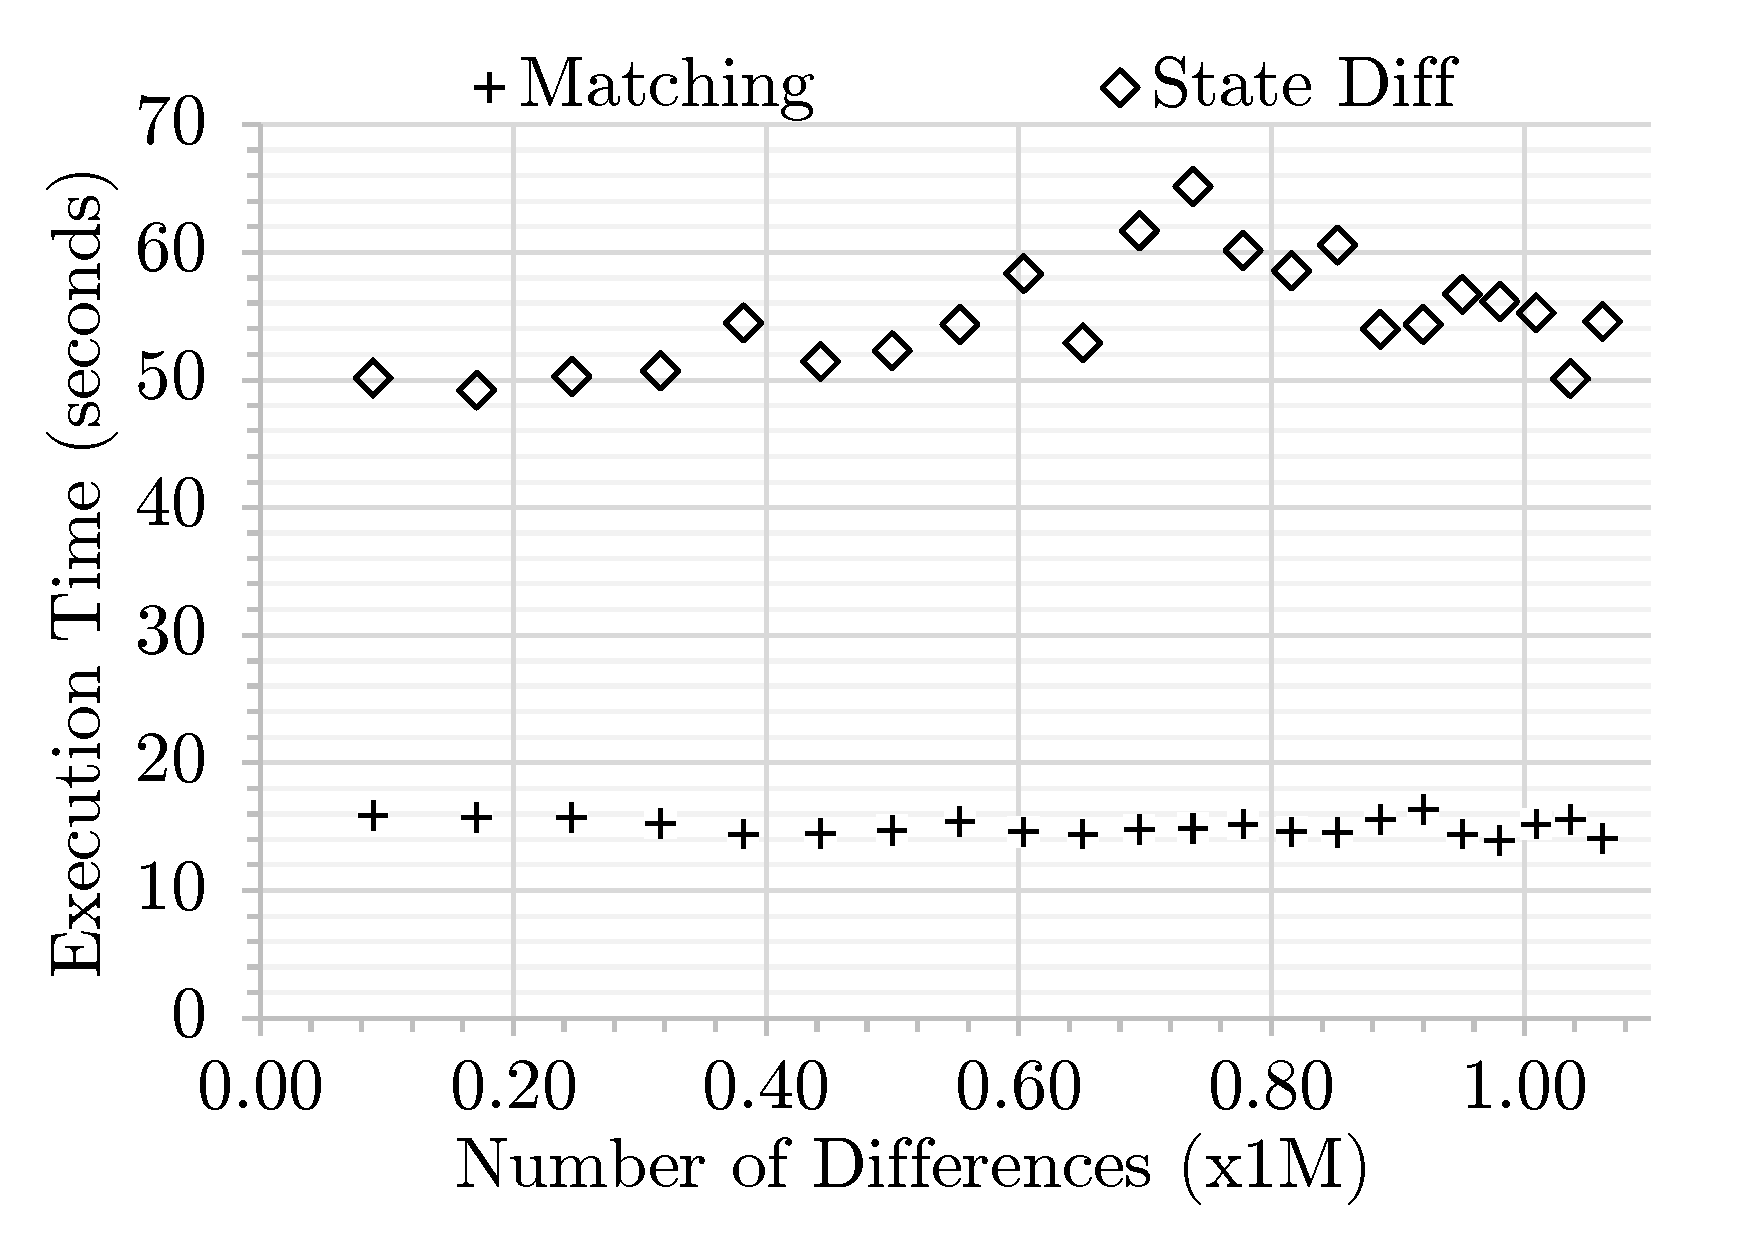
\includegraphics[width=\linewidth]{images/Time-StateDiff-Detail}
        \caption{state-based execution time}
        \label{fig:time_statediff_detail}
    \end{subfigure}
\begin{subfigure}[t]{0.495\linewidth}
    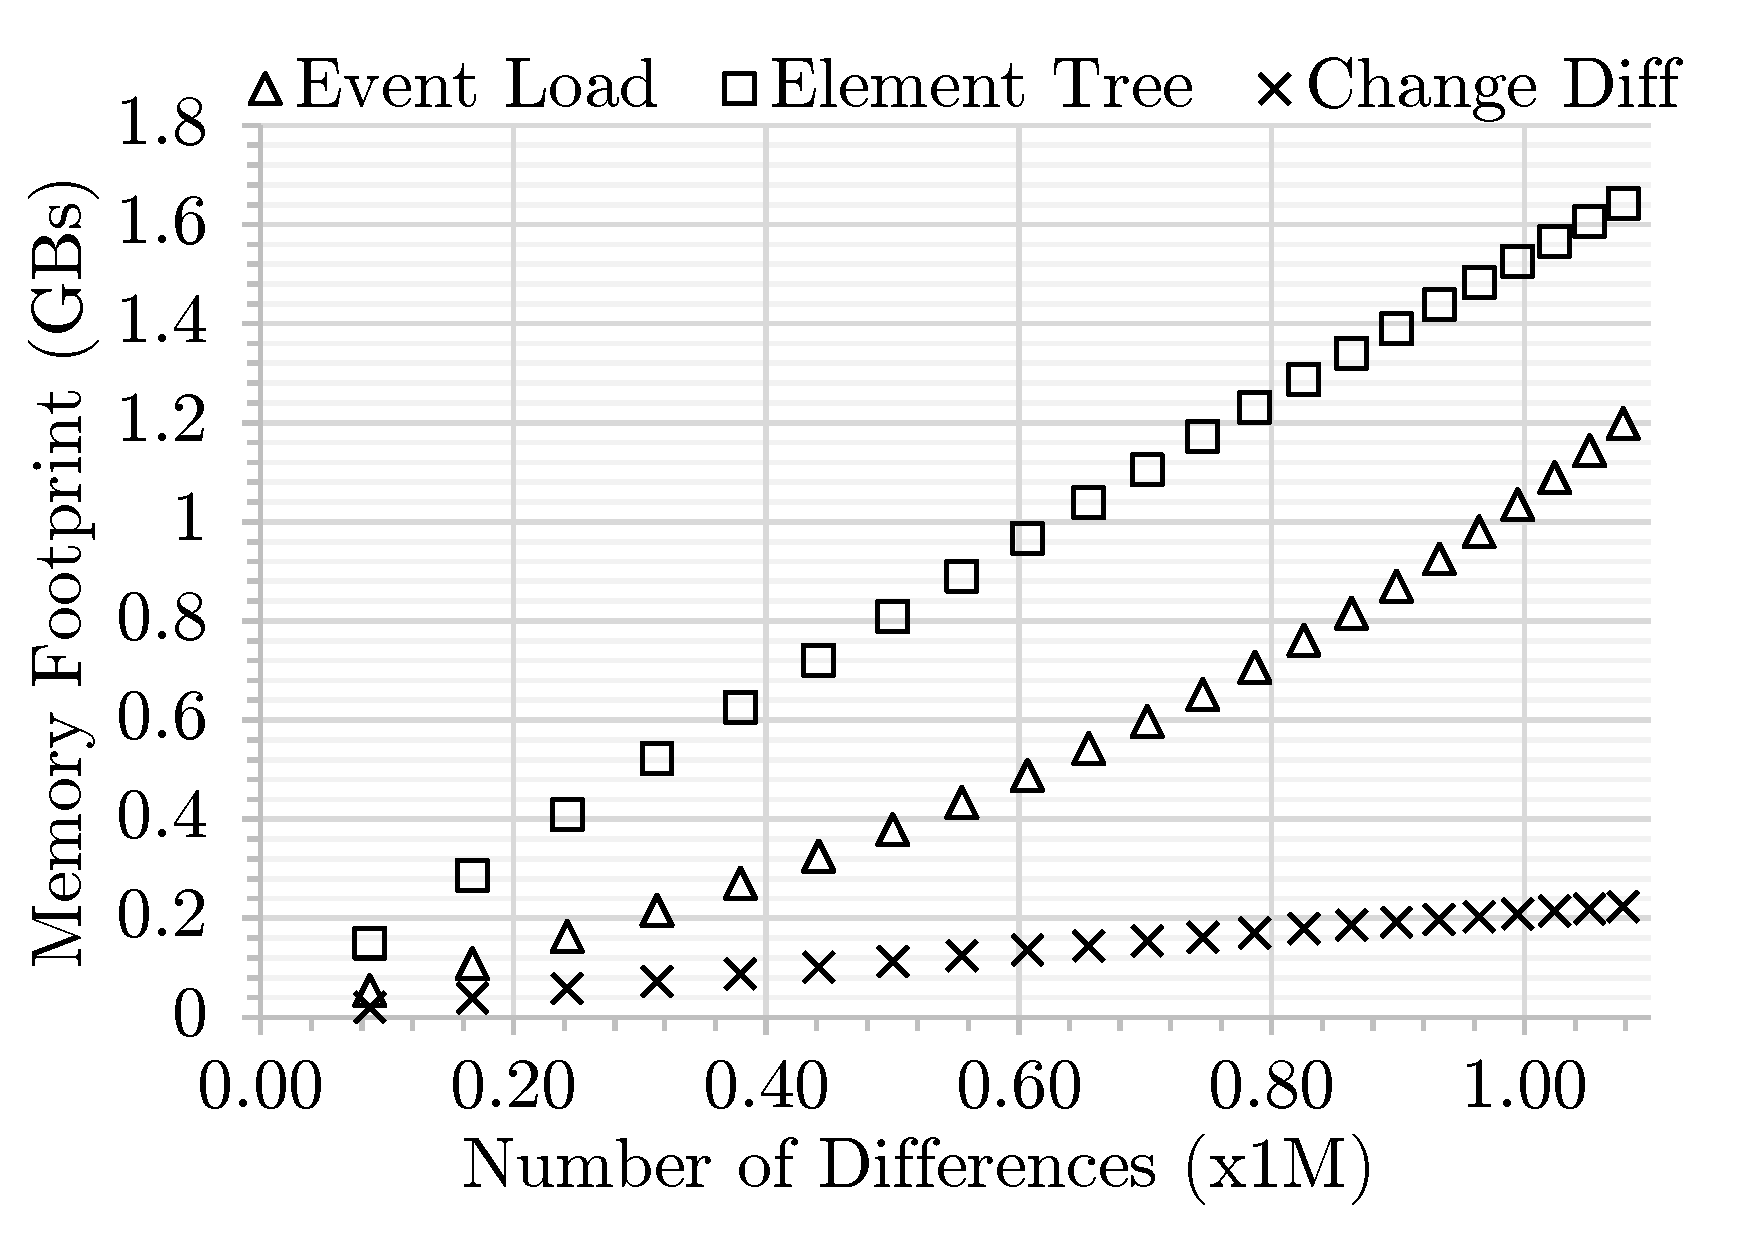
\includegraphics[width=\linewidth]{images/Memory-ChangeDiff-Detail}
    \caption{change-based memory footprint}
    \label{fig:memory_changediff_detail}
\end{subfigure}
\hfill
\begin{subfigure}[t]{0.495\linewidth}
    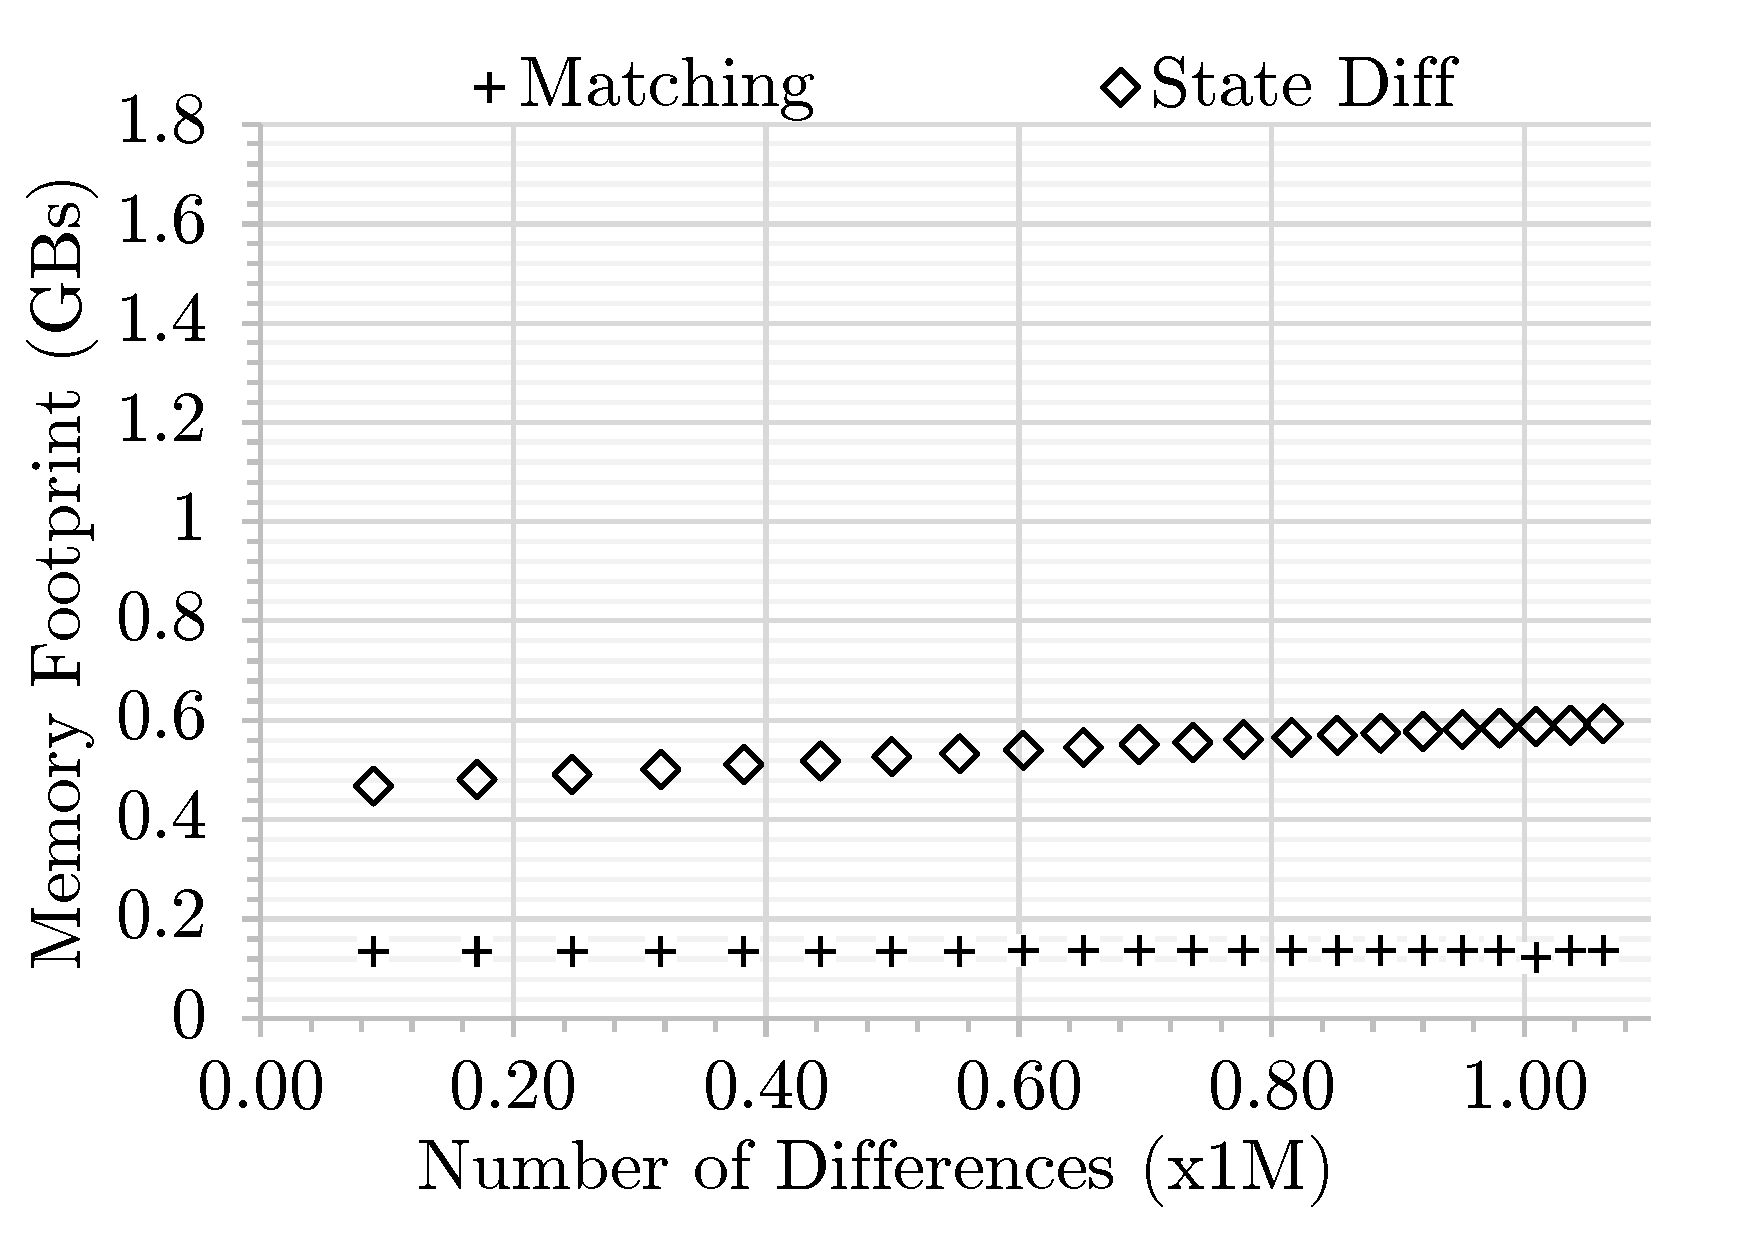
\includegraphics[width=\linewidth]{images/Memory-StateDiff-Detail}
    \caption{state-based memory footprint}
    \label{fig:memory_statediff_detail}
\end{subfigure}
    \caption{Breakdown view of execution time and memory in Figure \ref{fig:change_vs_state}.}
    \label{fig:time_memory_detail}
\end{figure}

For the state-based comparison in Fig. \ref{fig:time_statediff_detail}, the comparison time only experiences slight increase as the number of identified differences inclines. This slight increase is contributed mainly by the state-based diffing time while matching time tends to only contribute in constant due to the very small changes of the total elements (Figures \ref{fig:modification_course}, \ref{fig:model_size}).

Nevertheless, the change-based comparison also comes with a drawback on memory footprint since it consumes more space than the state-based comparison does (see Figure \ref{fig:memory_diffs}). Fig. \ref{fig:memory_changediff_detail} breaks down the memory footprint of the change-based comparison into three factors: the loaded change events, element tree, and diffs. As the number of differences grows, a great deal of events are generated. These events have to be loaded into memory since the information that they contain are important for the construction of the element tree. The memory used for these events grows exponentially against the number of differences since as the events increase some of these events do not contribute to the addition of new differences their memory space still needs to be retained. In our evaluation, the element tree occupies most of the memory footprint since it mimics the partial states -- elements and features -- of the models that are affected by the changes. In our technical implementation, a feature can have many instances -- one instance for each element (As a comparison, in the EMF implementation, there is only one instance for a feature. The feature is used as a key so that different elements can have the same feature that maps to different values simultaneously). This contributes to the large memory footprint used by the element three. The identified change-based diffs, the third factor, are the smallest factor that contributes to the memory footprint of the change-based comparison. 

For the state-based comparison in Fig. \ref{fig:memory_statediff_detail}, the memory footprint only inclines slightly along the increase of differences. Large part of the memory footprint are used to represent the identified differences, while the memory used for matches tends to be constant as the changes of the total elements are very small -- less new elements means less memory needs to be allocated for new matches (Figures \ref{fig:modification_course}, \ref{fig:model_size}). 

Based on the findings, we argue that the change-based comparison approach works at its best for large models that have been modified in a moderate number of changes. Models that have been excessively modified could impair the performance of change-based comparison as a great deal of change records have to be read and loaded into memory. 

\subsection{Limitation and Threat to Validity}
\label{sec:limitation_and_Threat_to_validity}

The proposed change-based comparison comes with a limitation that it heavily relies on the use of identifiers to efficiently address modified elements. Applying change-based persistent to models that use URI fragments as element's identifiers faces a challenge that an element's identifier is always changing when it is moved to another location in a model. The evaluation of the proposed change-based comparison is limited to the Java metamodel only. Thus, there is no guarantee it will always work on models with different metamodels. Although, we have tried to to cover as much as common changes made in EMF models (e.g. performing \textit{add}/\textit{remove}/\textit{set}/\textit{move} operations on \textit{single}/\textit{multi}-\textit{valued} features, \textit{attribute}/\textit{reference} features, or \textit{containment}/\textit{non}-\textit{containment} references), the random modification made in the evaluation does not largely reflect th evolution of models in the real-world. This is challenging as different domains can have their own patterns of model evolution -- different problems, metamodels, modellers, etc.

\section{Related Work}
\label{sec:related_work}
There are existing tools for model comparison. SiDiff \cite{Treude2007SiDiff} and DSMDiff \cite{lin2009dsmdiff} view models as graphs. They create matches and define differences between elements based on the similarity of their features. However, both are limited in flexibility to exploit the metamodel or particularities of a modelling language. EMF Compare \cite{emfcompare2018developer}, an established tool for model comparison and merging, addresses this by providing a extensible platform which users can define custom algorithms for matching, diffing, conflict detection, and merging. Flexibilty is also offered by ECL (Epsilon Comparison Language) \cite{kolovos2009ecl}, a hybrid, rule-based language for model comparison, which allows users to specify algorithms to match elements of homogeneous/heterogeneous models. All these tools work at structural level; they compare models based on their state-based features.

AMOR \cite{DBLP:conf/sfm/BroschKLSWW12}, a model versioning platform, also compares models in state-based. However, it also uses records of changes/operations of models to improve precision of conflict detection and resolution. For example, multiple conflicts caused by a composite operation should be resolved as one package, not as an individual conflict, to ensure consistency of resolution. EMFStore \cite{koegel2010emfstore} is a version control system for EMF models that stores model versions as packages of operations. Since it works purely in operations without considering the states of models, every operation is treated as a new change. Thus, concurrent operations that change a same feature to a same value are treated as conflicting operations. Moreover, owning its own version control system prevents users to use common textual version control systems (e.g. Git, SVN) for their models.  

%We differentiate our approach in that it compares two models by exploiting information available in their change records to identify differences in their states. Models are still persisted in change-based format. However, to speed up model comparison, our approach constructs only partial states of the models, thus reducing the scope of comparison only to elements affected by recent changes since the last version.   

\section{Conclusions and Future Work}
\label{sec:conclusion_and_future_work}
In this paper, we have proposed out approach to optimise model comparison by exploiting information contained in change-based persistence to localise comparison only to elements affected by recent changes. Our change-based persistence contains information that is enough to reconstruct an element tree -- a mapping of affected elements and features of models being compared. By iterating through elements and features in the element tree and comparing their values, positions, flags, etc., we can simply define their differences. Using such approach, we are able to produce model comparison that is more faster than traditional, state-based model comparison as shown in our evaluation. However, this approach also comes with a cost on memory footprint as it needs to load change events from a change-based persistence into main memory in order to operate. The next challenge for future work is to identify strategies to optimally merge models and persist the merging in change-based way. 

\vspace{-10pt}
\subsubsection*{Acknowledgements.} This work was partly supported by through a scholarship managed by \emph{Lembaga Pengelola Dana Pendidikan Indonesia} (Indonesia Endowment Fund for Education).
%\clearpage

\bibliography{references} 
\bibliographystyle{splncs}

\end{document} 
